% =========================================================================== %
% This is the main file for the Eclipse Scout book.
% 
% The technical latex setup and organisation of the book heavily borrows from
% "Pharo by Example" https://github.com/SquareBracketAssociates/PharoByExample-english 
% 
% =========================================================================== %
\documentclass[a4paper,10pt,twoside]{book}

% --------------------------------------------------------------------------- %
% definitions etc. common to all sub content
% --------------------------------------------------------------------------- %
%=============================================================================%
% Common things, settings, packages to include
%=============================================================================%

\usepackage{graphicx}
\usepackage{color}
\usepackage{makeidx}
\usepackage{ifpdf}
\usepackage{verbatim}

% --------------------------------------------------------------------------- %
% Setting up stuff depeding on output format
% --------------------------------------------------------------------------- %

\ifpdf
  % special settings for pdf mode
  \usepackage[colorlinks]{hyperref}
  \usepackage{courier}
  
  \hypersetup{
    colorlinks,
    linkcolor=darkblue,
    citecolor=darkblue,
    pdftitle={The Eclipse Scout Book},
    pdfauthor={The Scout Community},
    pdfkeywords={Enterprise Framework, Eclipse, Java, Client-Side, Rich Client, Web Client, Mobile},
    pdfsubject={Computer Science}
  }
  
  \usepackage{caption}
  \captionsetup{margin=10pt,font=small,labelfont=bf}
\else
  % special stuff for html mode
  \usepackage[tex4ht]{hyperref}
\fi

% --------------------------------------------------------------------------- %
% Setting up printing range
% --------------------------------------------------------------------------- %

\parindent 1cm
\parskip 0.2cm
\topmargin 0.2cm
\oddsidemargin 1cm
\evensidemargin 0.5cm
\textwidth 15cm
\textheight 21cm

% --------------------------------------------------------------------------- %
% Setting up listings
% --------------------------------------------------------------------------- %

\usepackage{listings}
 
\definecolor{darkviolet}{rgb}{0.5,0,0.4}
\definecolor{darkgreen}{rgb}{0,0.4,0.2} 
\definecolor{darkblue}{rgb}{0.1,0.1,0.9}
\definecolor{darkgrey}{rgb}{0.5,0.5,0.5}
\definecolor{lightblue}{rgb}{0.4,0.4,1}
\definecolor{lightgray}{rgb}{0.97,0.97,0.97}

\renewcommand{\lstlistlistingname}{List of Listings}

% general settings
\lstset{
  basicstyle=\small\ttfamily,
  columns=fullflexible,
  breaklines=true,
  breakindent=10pt,
  prebreak=\mbox{{\color{blue}\tiny$\searrow$}},
  postbreak=\mbox{{\color{blue}\tiny$\rightarrow$}},
  showstringspaces=false,
  backgroundcolor=\color{lightgray}
}

% settings for xml files
\lstdefinelanguage{xml}
{
  commentstyle=\color{darkgrey}\upshape,
  morestring=[b]",
  morestring=[s]{>}{<},
  morecomment=[s]{<?}{?>},
  stringstyle=\color{black},
  identifierstyle=\color{darkblue},
  keywordstyle=\color{cyan},
  morekeywords={xmlns,name,point,factory,class}% list your attributes here
}

% settings for ini files
\lstdefinelanguage{ini}
{
  morecomment=[f][\color{darkgrey}\upshape][0]\#, % # is comment iff it's the first char on the line
  stringstyle=\color{black}
}

% default settings (for java files)
\lstset{
  language=Java,
  emphstyle=\color{red}\bfseries,
  keywordstyle=\color{darkviolet}\bfseries,
  commentstyle=\color{darkgreen},
  morecomment=[s][\color{lightblue}]{/**}{*/},
  stringstyle=\color{darkblue},
}

% --------------------------------------------------------------------------- %
% cross reference macros
% --------------------------------------------------------------------------- %
\newcommand{\applabel}[1]{\label{apx:#1}}
\newcommand{\chalabel}[1]{\label{cha:#1}}
\newcommand{\seclabel}[1]{\label{sec:#1}}
\newcommand{\lstlabel}[1]{\label{lst:#1}}
\newcommand{\figlabel}[1]{\label{fig:#1}}
\newcommand{\tablabel}[1]{\label{tab:#1}}

\newcommand{\appref}[1]{Appendix~\ref{apx:#1}}
\newcommand{\charef}[1]{Chapter~\ref{cha:#1}\xspace}
\newcommand{\secref}[1]{Section~\ref{sec:#1}}
\newcommand{\lstref}[1]{Listing~\ref{lst:#1}\xspace}
\newcommand{\figref}[1]{Figure~\ref{fig:#1}\xspace}
\newcommand{\tabref}[1]{Table~\ref{tab:#1}\xspace}

% --------------------------------------------------------------------------- %
% graphics paths
% --------------------------------------------------------------------------- %
\graphicspath{
  {figures/}
  {Introduction/figures/}
}

%=============================================================================%


% --------------------------------------------------------------------------- %
% graphics paths
% --------------------------------------------------------------------------- %
\graphicspath{
  {figures/}
  {modules/figures/}
  {Introduction/figures/}
  {ScoutRuntime/figures/}
  {ScoutTooling/figures/}
  {OneDayTutorial/figures/}
  {ScoutClient/figures/}
  {ScoutInstallation/figures/}  
  {EclipseBasics/figures/}  
}

\let\wholebook=\relax
\makeindex

% --------------------------------------------------------------------------- %
% use this if you are working on individual chapters
% --------------------------------------------------------------------------- %
% \includeonly{Introduction/Introduction}
% \includeonly{ScoutRuntime/ScoutRuntime}

% =========================================================================== %
% Start content of book
% for usage of frontmatter etc. see
% http://tex.stackexchange.com/questions/20538/what-is-the-right-order-when-using-tableofcontents-frontmatter-mainmatter
% =========================================================================== %
\begin{document}

\ifpdf
  
\includepdf[pages=-]{ScoutBookCover.pdf}
\else
  
\includegraphics{ScoutBookCover.png}
\fi

\thispagestyle{empty}
\frontmatter

% --------------------------------------------------------------------------- %
% Title page, copyright, table of contents, preface
% --------------------------------------------------------------------------- %

%=============================================================================%
% The title page
%=============================================================================%

\author{Matthias Zimmermann}
\title{
\Huge\bf Eclipse Scout\\
\huge Frontend Development
}
\ifpdf
  \isodate
\fi
\date{\emph{Version of \today}}
\maketitle

%=============================================================================%


\pagenumbering{roman}
\pagestyle{plain}

\tableofcontents
\sloppy

% =========================================================================== %
% Preface
% please make sure that this fits into two pages (max)
% =========================================================================== %

\ifx\wholebook\relax\else
  \documentclass[a4paper,10pt,twoside]{book}
  %=============================================================================%
% Common things, settings, packages to include
%=============================================================================%

\usepackage{graphicx}
\usepackage{color}
\usepackage{makeidx}
\usepackage{ifpdf}
\usepackage{verbatim}

% --------------------------------------------------------------------------- %
% Setting up stuff depeding on output format
% --------------------------------------------------------------------------- %

\ifpdf
  % special settings for pdf mode
  \usepackage[colorlinks]{hyperref}
  \usepackage{courier}
  
  \hypersetup{
    colorlinks,
    linkcolor=darkblue,
    citecolor=darkblue,
    pdftitle={The Eclipse Scout Book},
    pdfauthor={The Scout Community},
    pdfkeywords={Enterprise Framework, Eclipse, Java, Client-Side, Rich Client, Web Client, Mobile},
    pdfsubject={Computer Science}
  }
  
  \usepackage{caption}
  \captionsetup{margin=10pt,font=small,labelfont=bf}
\else
  % special stuff for html mode
  \usepackage[tex4ht]{hyperref}
\fi

% --------------------------------------------------------------------------- %
% Setting up printing range
% --------------------------------------------------------------------------- %

\parindent 1cm
\parskip 0.2cm
\topmargin 0.2cm
\oddsidemargin 1cm
\evensidemargin 0.5cm
\textwidth 15cm
\textheight 21cm

% --------------------------------------------------------------------------- %
% Setting up listings
% --------------------------------------------------------------------------- %

\usepackage{listings}
 
\definecolor{darkviolet}{rgb}{0.5,0,0.4}
\definecolor{darkgreen}{rgb}{0,0.4,0.2} 
\definecolor{darkblue}{rgb}{0.1,0.1,0.9}
\definecolor{darkgrey}{rgb}{0.5,0.5,0.5}
\definecolor{lightblue}{rgb}{0.4,0.4,1}
\definecolor{lightgray}{rgb}{0.97,0.97,0.97}

\renewcommand{\lstlistlistingname}{List of Listings}

% general settings
\lstset{
  basicstyle=\small\ttfamily,
  columns=fullflexible,
  breaklines=true,
  breakindent=10pt,
  prebreak=\mbox{{\color{blue}\tiny$\searrow$}},
  postbreak=\mbox{{\color{blue}\tiny$\rightarrow$}},
  showstringspaces=false,
  backgroundcolor=\color{lightgray}
}

% settings for xml files
\lstdefinelanguage{xml}
{
  commentstyle=\color{darkgrey}\upshape,
  morestring=[b]",
  morestring=[s]{>}{<},
  morecomment=[s]{<?}{?>},
  stringstyle=\color{black},
  identifierstyle=\color{darkblue},
  keywordstyle=\color{cyan},
  morekeywords={xmlns,name,point,factory,class}% list your attributes here
}

% settings for ini files
\lstdefinelanguage{ini}
{
  morecomment=[f][\color{darkgrey}\upshape][0]\#, % # is comment iff it's the first char on the line
  stringstyle=\color{black}
}

% default settings (for java files)
\lstset{
  language=Java,
  emphstyle=\color{red}\bfseries,
  keywordstyle=\color{darkviolet}\bfseries,
  commentstyle=\color{darkgreen},
  morecomment=[s][\color{lightblue}]{/**}{*/},
  stringstyle=\color{darkblue},
}

% --------------------------------------------------------------------------- %
% cross reference macros
% --------------------------------------------------------------------------- %
\newcommand{\applabel}[1]{\label{apx:#1}}
\newcommand{\chalabel}[1]{\label{cha:#1}}
\newcommand{\seclabel}[1]{\label{sec:#1}}
\newcommand{\lstlabel}[1]{\label{lst:#1}}
\newcommand{\figlabel}[1]{\label{fig:#1}}
\newcommand{\tablabel}[1]{\label{tab:#1}}

\newcommand{\appref}[1]{Appendix~\ref{apx:#1}}
\newcommand{\charef}[1]{Chapter~\ref{cha:#1}\xspace}
\newcommand{\secref}[1]{Section~\ref{sec:#1}}
\newcommand{\lstref}[1]{Listing~\ref{lst:#1}\xspace}
\newcommand{\figref}[1]{Figure~\ref{fig:#1}\xspace}
\newcommand{\tabref}[1]{Table~\ref{tab:#1}\xspace}

% --------------------------------------------------------------------------- %
% graphics paths
% --------------------------------------------------------------------------- %
\graphicspath{
  {figures/}
  {Introduction/figures/}
}

%=============================================================================%

	\pagestyle{headings}
  \graphicspath{{figures/} {../figures/}}
  \begin{document}
  \sloppy
\fi


% --------------------------------------------------------------------------- %
\chapter{Preface}

Today, the Java platform is widely seen as the primary choice for implementing enterprise applications. 
While many successful frameworks support the development of persistence layers and business services, implementing front-ends in a simple and clean way remains a challenge. 
This is exactly where Eclipse Scout fits in. 
The primary goal of Scout is to make your life as a developer easier and to help organisations to save money and time. 
For this, the Scout framework covers most of the recurring front-end aspects such as user authentication, client-server communication and the user interface. 
This comprehensive scope reduces the amount of necessary boiler plate code, and let developers concentrate on understanding and implementing business functionality. 

The purpose of this book is to get the reader familiar with the Scout framework.
In this book Scout's core features are introduced and explained using many practical examples. 
And as both the Scout framework and Scout applications are written in Java, we make the assumption that you are familiar with the language too. 
Ideally, you have worked with Java for some time now and feel comfortable with the basic language features. 

In the first part of the book a general introduction into the runtime part of the framework and the tooling - the Scout SDK - is provided. 
After the mandatory ''Hello World!'' application, the book walks you though a complete client server application including database access. 
The focus of the book's second part is on the front-end side of Scout applications. 
First, an overview of the Scout client model is introduced before Scout's most important UI components are described based on the Scout widget demo application. 
To cover the the server-side of Scout applications, an additional part of the book is planned to be released jointly with version 5.0 of the Scout framework. 
And finally, we intend to amend the book regarding building, testing and continuous integration for Scout applications. 

Last but not least, we thank you for your interest in Scout, for being part of our community and for your friendly support of new community members.
To allow for contributions to this book, the technical setup and the book's licence have been selected to minimize restrictions. 
According to the terms of the Creative Commons (CC-BY) license, you are allowed to freely use, share and adapt this book. 
All source files of the book including the Scout projects described in the book are available on github.
For the first edition of this book, we did already receive a number of bug reports and comments that were pointing out mistakes, inconsistencies and suggestions for changes. 
This feedback is very valuable to us as it helps to improve both the book's content and the quality for all future readers. 
We hope that this book helps you to get started quickly and would love to get your feedback. 

% --------------------------------------------------------------------------- %

\ifx\wholebook\relax\else
   \begin{thebibliography}{99}
  \addcontentsline{toc}{chapter}{Bibliography}
  
  % add/insert books in alphabetical order of 1st author
  
  \bibitem{batessierra05}
    \textit{Bert Bates, Kathy Sierra},
	\textbf{Head First Java} 2nd edition, 
	O'Reilly Media, 2005.

  \bibitem{bloch08} 
    \textit{Joshua Bloch},
    \textbf{Effective Java} 2nd edition, 
	Addison-Wesley, 2008.
	
  \bibitem{eckel06}
    \textit{Bruce Eckel},
	\textbf{Thinking in Java} 4th edition, 
	Prentice Hall International, 2006.

\end{thebibliography}

   \end{document}
\fi

% =========================================================================== %

\mainmatter

% =========================================================================== %
% Main content of book starts here
% =========================================================================== %

\pagestyle{headings}
\pagenumbering{arabic}

% --------------------------------------------------------------------------- %
% =========================================================================== %
% The Scout Client
% =========================================================================== %

\ifx\wholebook\relax\else
  \documentclass[a4paper,10pt,twoside]{book}
  %=============================================================================%
% Common things, settings, packages to include
%=============================================================================%

\usepackage{graphicx}
\usepackage{color}
\usepackage{makeidx}
\usepackage{ifpdf}
\usepackage{verbatim}

% --------------------------------------------------------------------------- %
% Setting up stuff depeding on output format
% --------------------------------------------------------------------------- %

\ifpdf
  % special settings for pdf mode
  \usepackage[colorlinks]{hyperref}
  \usepackage{courier}
  
  \hypersetup{
    colorlinks,
    linkcolor=darkblue,
    citecolor=darkblue,
    pdftitle={The Eclipse Scout Book},
    pdfauthor={The Scout Community},
    pdfkeywords={Enterprise Framework, Eclipse, Java, Client-Side, Rich Client, Web Client, Mobile},
    pdfsubject={Computer Science}
  }
  
  \usepackage{caption}
  \captionsetup{margin=10pt,font=small,labelfont=bf}
\else
  % special stuff for html mode
  \usepackage[tex4ht]{hyperref}
\fi

% --------------------------------------------------------------------------- %
% Setting up printing range
% --------------------------------------------------------------------------- %

\parindent 1cm
\parskip 0.2cm
\topmargin 0.2cm
\oddsidemargin 1cm
\evensidemargin 0.5cm
\textwidth 15cm
\textheight 21cm

% --------------------------------------------------------------------------- %
% Setting up listings
% --------------------------------------------------------------------------- %

\usepackage{listings}
 
\definecolor{darkviolet}{rgb}{0.5,0,0.4}
\definecolor{darkgreen}{rgb}{0,0.4,0.2} 
\definecolor{darkblue}{rgb}{0.1,0.1,0.9}
\definecolor{darkgrey}{rgb}{0.5,0.5,0.5}
\definecolor{lightblue}{rgb}{0.4,0.4,1}
\definecolor{lightgray}{rgb}{0.97,0.97,0.97}

\renewcommand{\lstlistlistingname}{List of Listings}

% general settings
\lstset{
  basicstyle=\small\ttfamily,
  columns=fullflexible,
  breaklines=true,
  breakindent=10pt,
  prebreak=\mbox{{\color{blue}\tiny$\searrow$}},
  postbreak=\mbox{{\color{blue}\tiny$\rightarrow$}},
  showstringspaces=false,
  backgroundcolor=\color{lightgray}
}

% settings for xml files
\lstdefinelanguage{xml}
{
  commentstyle=\color{darkgrey}\upshape,
  morestring=[b]",
  morestring=[s]{>}{<},
  morecomment=[s]{<?}{?>},
  stringstyle=\color{black},
  identifierstyle=\color{darkblue},
  keywordstyle=\color{cyan},
  morekeywords={xmlns,name,point,factory,class}% list your attributes here
}

% settings for ini files
\lstdefinelanguage{ini}
{
  morecomment=[f][\color{darkgrey}\upshape][0]\#, % # is comment iff it's the first char on the line
  stringstyle=\color{black}
}

% default settings (for java files)
\lstset{
  language=Java,
  emphstyle=\color{red}\bfseries,
  keywordstyle=\color{darkviolet}\bfseries,
  commentstyle=\color{darkgreen},
  morecomment=[s][\color{lightblue}]{/**}{*/},
  stringstyle=\color{darkblue},
}

% --------------------------------------------------------------------------- %
% cross reference macros
% --------------------------------------------------------------------------- %
\newcommand{\applabel}[1]{\label{apx:#1}}
\newcommand{\chalabel}[1]{\label{cha:#1}}
\newcommand{\seclabel}[1]{\label{sec:#1}}
\newcommand{\lstlabel}[1]{\label{lst:#1}}
\newcommand{\figlabel}[1]{\label{fig:#1}}
\newcommand{\tablabel}[1]{\label{tab:#1}}

\newcommand{\appref}[1]{Appendix~\ref{apx:#1}}
\newcommand{\charef}[1]{Chapter~\ref{cha:#1}\xspace}
\newcommand{\secref}[1]{Section~\ref{sec:#1}}
\newcommand{\lstref}[1]{Listing~\ref{lst:#1}\xspace}
\newcommand{\figref}[1]{Figure~\ref{fig:#1}\xspace}
\newcommand{\tabref}[1]{Table~\ref{tab:#1}\xspace}

% --------------------------------------------------------------------------- %
% graphics paths
% --------------------------------------------------------------------------- %
\graphicspath{
  {figures/}
  {Introduction/figures/}
}

%=============================================================================%

  \pagestyle{headings}
  \graphicspath{{figures/} {../figures/}}
  \begin{document}
  \sloppy
\fi


% =========================================================================== %
\chapter{Overview}
\chalabel{client_overview}

needs text
  
\noindent Existing Documentation
\begin{itemize}
  \item concept wiki \url{http://wiki.eclipse.org/Scout/Concepts/Client_Plug-In}
\end{itemize}

% --------------------------------------------------------------------------- %
\section{Component Model}
needs text

\noindent Existing Documentation
\begin{itemize}
  \item wiki concept \url{http://wiki.eclipse.org/Scout/Concepts/Client_Plug-In#Component_Model}
  \item concept wiki \url{http://wiki.eclipse.org/Scout/Concepts/ClientSession}
\end{itemize}

  * client session
  * ui
  * other
  
% --------------------------------------------------------------------------- %
\section{Separation of UI Technologies}
needs text

\noindent Existing Documentation
\begin{itemize}
  \item wiki concept \url{http://wiki.eclipse.org/Scout/Concepts/Client_Plug-In#Separation_of_UI_and_GUI}
\end{itemize}
  
  * swing
  * swt
  * rap

\section{Test for Listing}

introductionary listing

\lstinputlisting[
  caption=The DesktopForm.java in the UI,
]
{../code/helloworld/org.eclipse.scout.helloworld.client/src/org/eclipse/scout/helloworld/client/ui/forms/DesktopForm.java}


some text before listing\index{listing} \ref{samplecode}.

\lstinputlisting[
  label=samplecode,
  caption=The HelloWorld.java sample with emphasys on \it{println},
  index={println,main,String},
  float,
  emph={println}
]
{../code/helloworldJava/HelloWorld.java}


\lstinputlisting[
  label=samplecode-main,
  caption=Snippet containing the main method,
  linerange={14-18},
  float
]
{../code/helloworldJava/HelloWorld.java}


some text after listing \ref{samplecode} and \ref{samplecode-main}.

% =========================================================================== %
\chapter{Client Modeling}
\chalabel{client_modeling}

needs text. this should be a complete chapter as the client modeling is one
of scouts key features.

internal structure to be decided. consequences for other chapters/sections in
this part to be verified

% =========================================================================== %
\chapter{Shared Components}
needs text
  
% --------------------------------------------------------------------------- %
\section{Texts / i18n / NLS Support}
needs text

\noindent Existing Documentation
\begin{itemize}
  \item concept wiki: \url{http://wiki.eclipse.org/Scout/Concepts/Texts}
  \item forum: \url{http://www.eclipse.org/forums/index.php/t/319136/}
  \item forum: \url{http://www.eclipse.org/forums/index.php/t/326343/}
  \item forum: overwriting texts provided by scout \url{http://www.eclipse.org/forums/index.php/t/308273/}
  \item forum: additional text provider service \url{http://www.eclipse.org/forums/index.php/t/317565/}
  \item forum: changing default language for scout apps \url{http://www.eclipse.org/forums/index.php/t/367177/}
  \item forum: export/import not possible: \url{http://www.eclipse.org/forums/index.php/t/326320/}
  \item forum: usage counts for text entries: \url{http://www.eclipse.org/forums/index.php/t/261235/}
\end{itemize}

\begin{lstlisting}[
  float,
  caption=A floating HelloWorld example,
  index={main},
  gobble=2
]
    /*************************************************
     * main method
     *************************************************/
    public static void main(String[] args) {
        // some normal line comment
        System.out.println("Hello, World");
        Some.big().andEspeciallyLong().getThisOrThat().orSomething("string", null).doThis().doThat;
    }
\end{lstlisting}

% --------------------------------------------------------------------------- %
\section{Icons}
needs text

\noindent Existing Documentation
\begin{itemize}
  \item how-to wiki \url{http://wiki.eclipse.org/Scout/HowTo/3.8/Add_an_icon}
  \item how-to wiki \url{http://wiki.eclipse.org/Scout/HowTo/3.8/Exchange_Default_Images}
\end{itemize}

% --------------------------------------------------------------------------- %
\section{Codes and Code Types}
needs text

\noindent Existing Documentation
\begin{itemize}
  \item how-to wiki: \url{http://wiki.eclipse.org/Scout/Tutorial/3.8/Minicrm/Code_Types}
  \item concept wiki \url{http://wiki.eclipse.org/Scout/Concepts/CodeType}
  \item forum: codes from database \url{http://www.eclipse.org/forums/index.php/t/282531/}
\end{itemize}

  * codes and codetypes
  * static code types
  * dynamic code types
  * hierarchical code types

  
  
\lstinputlisting[
  language=xml,
  label=samplecode-xml,
  caption=The \tt{plugin.xml} file,
  float
]
{../code/helloworldJava/xml/plugin.xml}

and then some listing with the config.ini.

\lstinputlisting[
  language=ini,
  label=samplecode-ini,
  caption=The \tt{config.ini} file
]
{../code/helloworldJava/ini/config.ini}

% --------------------------------------------------------------------------- %
\section{Lookup Calls and Services}
needs text
 
\noindent Existing Documentation
\begin{itemize}
  \item presentation: \url{http://wiki.eclipse.org/images/c/c9/20111102_EclipseConEurope2011-EclipseScout-DiscoverThePotential.pdf}
  \item concept wiki: \url{http://wiki.eclipse.org/Scout/Concepts/LookupCall}
  \item forum: \url{http://www.eclipse.org/forums/index.php/t/279108/}
\end{itemize}

    * lookup call
  * lookup service
  * sqllookup service

% --------------------------------------------------------------------------- %
\section{Permissions}

needs text, topic is relevant for client, server, and security. what to present where to be decided

\noindent Existing Documentation
\begin{itemize}
  \item how-to wiki: \url{http://wiki.eclipse.org/Scout/HowTo/3.8/Create_Permissions}
  \item concept wiki: \url{http://wiki.eclipse.org/Scout/Concepts/Permission}
  \item forum: \url{http://www.eclipse.org/forums/index.php/t/243966/}
\end{itemize}

% --------------------------------------------------------------------------- %
\section{Form Data Objects}
needs text, explain that form data objects are data transfer objects

\noindent Existing Documentation
\begin{itemize}
  \item form data/dto \url{http://www.eclipse.org/forums/index.php/t/169334/}
\end{itemize}

\subsection{Data Binding}
needs text, this is about Form Data Export and Import

\subsection{Automatic Updates by the Scout SDK}
needs text

\subsection{Manual Form Data Updates}
needs text

% =========================================================================== %
\chapter{Client components}
needs text

% --------------------------------------------------------------------------- %
\section{Splash Screen}
needs text

% --------------------------------------------------------------------------- %
\section{Login Box}
needs text

% --------------------------------------------------------------------------- %
\section{Client Session}
needs text

% --------------------------------------------------------------------------- %
\section{Desktop}
needs text

\noindent Existing Documentation
\begin{itemize}
  \item concept wiki \url{http://wiki.eclipse.org/Scout/Concepts/Desktop}
\end{itemize}

\subsection{Info Dialog}
needs text

\subsection{Toolbar}
needs text

\noindent Existing Documentation
\begin{itemize}
  \item forum: feature request \url{http://www.eclipse.org/forums/index.php/t/366440/}
  \item concept wiki \url{http://wiki.eclipse.org/Scout/Concepts/Tool}
\end{itemize}

\subsection{Status Line}
needs text

% --------------------------------------------------------------------------- %
\section{Menus}
needs text

\noindent Existing Documentation
\begin{itemize}
  \item concept wiki \url{http://wiki.eclipse.org/Scout/Concepts/Menu}
  \item forum: hard coded swt menues \url{http://www.eclipse.org/forums/index.php/t/236071/}. is this still an issue with scout kepler?
\end{itemize}

% --------------------------------------------------------------------------- %
\section{Outlines}
needs text

\noindent Existing Documentation
\begin{itemize}
  \item concept wiki \url{http://wiki.eclipse.org/Scout/Concepts/Outline}
\end{itemize}

% --------------------------------------------------------------------------- %
\section{Tools}
needs text

	
% --------------------------------------------------------------------------- %
\section{Forms}
needs text

\noindent Existing Documentation
\begin{itemize}
  \item concept wiki \url{http://wiki.eclipse.org/Scout/Concepts/Form}
  \item concept wiki form handler\url{http://wiki.eclipse.org/Scout/Concepts/Form_Handler}
  \item how-to wiki \url{http://wiki.eclipse.org/Scout/HowTo/3.8/Open_a_Form_in_a_View}
  \item forum: layout manager \url{http://www.eclipse.org/forums/index.php/t/404048/}
  \item forum: life cycle \url{http://www.eclipse.org/forums/index.php/t/369890/}
\end{itemize}

	* form validation

% --------------------------------------------------------------------------- %
\section{Trees}
needs text

    * tree nodes
	* tree form
	* tree field

% --------------------------------------------------------------------------- %
\section{Pages}
needs text

\noindent Existing Documentation
\begin{itemize}
  \item how-to wiki: \url{http://wiki.eclipse.org/Scout/HowTo/3.8/Display_images_in_a_table_page}	
  \item concept wiki: \url{http://wiki.eclipse.org/Scout/Concepts/Page}
  \item forum: pages linking to forms \url{http://www.eclipse.org/forums/index.php/t/367595/}
  \item forum: changing page icons \url{http://www.eclipse.org/forums/index.php/t/262151/}
\end{itemize}

    * page with table
	* page with nodes

	
% --------------------------------------------------------------------------- %
\section{Search Forms}
needs text

\noindent Existing Documentation
\begin{itemize}
  \item forum: position of search form \url{http://www.eclipse.org/forums/index.php/t/353895/}
  \item forum: statement builder stuff \url{http://www.eclipse.org/forums/index.php/t/165805/}
\end{itemize}
	
% --------------------------------------------------------------------------- %
\section{Tables}
needs text

\noindent Existing Documentation
\begin{itemize}
  \item forum: editable column \url{http://www.eclipse.org/forums/index.php/t/220019/}
  \item forum: default visibility of columns \url{http://www.eclipse.org/forums/index.php/t/166052/}
  \item forum: row deletion \url{http://www.eclipse.org/forums/index.php/t/210744/}
\end{itemize}

	* context menues
	* editable tables
    * column types

\subsection{Image Columns}
needs text

\noindent Existing Documentation
\begin{itemize}
  \item forum: \url{http://www.eclipse.org/forums/index.php/t/369626/}
\end{itemize}

\subsection{HTML inside Table Cells}
needs text

\noindent Existing Documentation
\begin{itemize}
  \item forum: \url{http://www.eclipse.org/forums/index.php/t/370714/}
  \item forum: summary row \url{http://www.eclipse.org/forums/index.php/t/235749/}
\end{itemize}

\subsection{Table Status Bar}
nees text

\noindent Existing Documentation
\begin{itemize}
  \item forum: \url{http://www.eclipse.org/forums/index.php/t/367326/}
\end{itemize}

\subsection{Injecting Columns at Runtime}
needs text

\noindent Existing Documentation
\begin{itemize}
  \item forum: \url{http://www.eclipse.org/forums/index.php/t/364715/}
  \item forum : dynamic columns \url{http://www.eclipse.org/forums/index.php/t/216731/}
\end{itemize}

% --------------------------------------------------------------------------- %
\section{Workflows and Wizards}
Needs text

\noindent Existing Documentation
\begin{itemize}
  \item concept wiki \url{http://wiki.eclipse.org/Scout/Concepts/Wizard}
  \item forum: \url{http://www.eclipse.org/forums/index.php/t/391607/}
  \item forum: \url{http://www.eclipse.org/forums/index.php/t/382579/}
  \item forum: \url{http://www.eclipse.org/forums/index.php/t/366971/}
\end{itemize}




% =========================================================================== %
\chapter{Layouting}
needs text

\noindent Existing Documentation
\begin{itemize}
  \item concept wiki \url{http://wiki.eclipse.org/Scout/Concepts/Client_Plug-In#Layouting}
\end{itemize}

% --------------------------------------------------------------------------- %
\section{The Desktop}
needs text

% --------------------------------------------------------------------------- %
\section{The Stuff in the Middle}
needs text

% --------------------------------------------------------------------------- %
\section{Form Layout}
needs text

% =========================================================================== %
\chapter{Form Fields}
\chalabel{fields}

needs text

\noindent Existing Documentation
\begin{itemize}
  \item concept wiki (links) \url{http://wiki.eclipse.org/Scout/Concepts/Client_Plug-In#Form_fields}
  \item concept wiki screenshots \url{http://wiki.eclipse.org/Scout/Concepts/Field}
\end{itemize}

% --------------------------------------------------------------------------- %
\section{Common Aspects}
needs text

\noindent Existing Documentation
\begin{itemize}
  \item forum: label position \url{http://www.eclipse.org/forums/index.php/t/369109/}
\end{itemize}

* exec methods
* field validation

	
% --------------------------------------------------------------------------- %
\section{Grouping Components}
needs text

* layouting
* group box
* tab box
* sequence box 
* split box

% --------------------------------------------------------------------------- %
\section{Group Box}
needs text

% --------------------------------------------------------------------------- %
\section{Tab Box}
needs text

% --------------------------------------------------------------------------- %
\section{Sequence Box}
needs text

\noindent Existing Documentation
\begin{itemize}
  \item forum: \url{http://www.eclipse.org/forums/index.php/t/414629/}
\end{itemize}

* exec methods
* field validation


% --------------------------------------------------------------------------- %
\section{Split Box}
needs text

% --------------------------------------------------------------------------- %
\section{Radio Button Group}
needs text

\noindent Existing Documentation
\begin{itemize}
  \item forum: \url{http://www.eclipse.org/forums/index.php/t/366324/}
\end{itemize}

% --------------------------------------------------------------------------- %
\section{Label Field}
needs text
	
% --------------------------------------------------------------------------- %
\section{String Field}
needs text

\noindent Existing Documentation
\begin{itemize}
  \item forum: \url{http://www.eclipse.org/forums/index.php/t/369263/}
  \item forum: validation on any key \url{http://www.eclipse.org/forums/index.php/t/198123/}
\end{itemize}

% --------------------------------------------------------------------------- %
\section{Integer Field}
needs text
	
% --------------------------------------------------------------------------- %
\section{Number Field}
needs text
	
% --------------------------------------------------------------------------- %
\section{Date Field}
needs text

% --------------------------------------------------------------------------- %
\section{Button Field}
needs text

% --------------------------------------------------------------------------- %
\section{Link Field}
needs text

% --------------------------------------------------------------------------- %
\section{Smart Field}
needs text

\noindent Existing Documentation
\begin{itemize}
  \item presentation: \url{http://wiki.eclipse.org/images/c/c9/20111102_EclipseConEurope2011-EclipseScout-DiscoverThePotential.pdf}
  \item forum: \url{http://www.eclipse.org/forums/index.php/t/369542/}
\end{itemize}

\subsection{Menus}
Each smart field can have menus attached. The menus will be shown when the user clicks on the \emph{arrow} symbol next to the smart field. Figure \ref{fig:smartfield_menu} shows an example of a smart field along with a set of menus.
\begin{figure}[!htb]
\centering
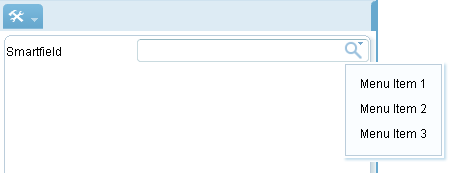
\includegraphics[width=0.8\textwidth]{smartfieldmenu.png}
\caption{Menus attached to a smart field.}
\label{fig:smartfield_menu}
\end{figure}

By default, the menus will only be shown if a value of the smart field has been selected. To show the menus even if the smart field is empty, one has to override the menu's \lstinline$getConfiguredEmptySpaceAction$ method:

\begin{lstlisting}[backgroundcolor=\color{white}]
@Override
protected boolean getConfiguredEmptySpaceAction() {
 return true;
}
\end{lstlisting}

% --------------------------------------------------------------------------- %
\section{List Box}
needs text

% --------------------------------------------------------------------------- %
\section{Tree Box}
needs text

% --------------------------------------------------------------------------- %
\section{Table Field}
needs text

\noindent Existing Documentation
\begin{itemize}
  \item wiki tutorial \url{http://wiki.eclipse.org/Scout/Tutorial/3.8/Minicrm/Table_Field}
  \item forum: \url{http://www.eclipse.org/forums/index.php/t/392053/}
  \item forum: load/save data \url{http://www.eclipse.org/forums/index.php/t/253311/}
\end{itemize}

% --------------------------------------------------------------------------- %
\section{Page Field}
needs text

\noindent Existing Documentation
\begin{itemize}
  \item forum: \url{http://www.eclipse.org/forums/index.php/t/395360/}
\end{itemize}

% --------------------------------------------------------------------------- %
\section{Image Field}
needs text

\noindent Existing Documentation
\begin{itemize}
  \item forum: scrollbars \url{http://www.eclipse.org/forums/index.php/t/291205/}
\end{itemize}

% --------------------------------------------------------------------------- %
\section{HTML Field}
needs text

% --------------------------------------------------------------------------- %
\section{Image Field}
needs text

% --------------------------------------------------------------------------- %
\section{SVG Field}
needs text

\noindent Existing Documentation
\begin{itemize}
  \item wiki tutorial \url{http://wiki.eclipse.org/Scout/Tutorial/3.8/SVG_Field}
\end{itemize}

% --------------------------------------------------------------------------- %
\section{Browser Field}
needs text

\noindent Existing Documentation
\begin{itemize}
  \item forum: \url{http://www.eclipse.org/forums/index.php/t/414483/}, 
  \item forum: \url{http://www.eclipse.org/forums/index.php/t/369963/}, 
  \item forum: mozilla as default: \url{http://www.eclipse.org/forums/index.php/t/342433/}
\end{itemize}

% --------------------------------------------------------------------------- %
\section{Calendar Field}
needs text

\noindent Existing Documentation
\begin{itemize}
  \item forum: calendar field \url{http://www.eclipse.org/forums/index.php/t/370052/}
  \item forum: execloaditems \url{http://www.eclipse.org/forums/index.php/t/277447/}
  \item forum: filtering items \url{http://www.eclipse.org/forums/index.php/t/285644/}
  \item forum: usage example \url{http://www.eclipse.org/forums/index.php/t/265028/}
\end{itemize}

% --------------------------------------------------------------------------- %
\section{File Chooser Field}
needs text

\noindent Existing Documentation
\begin{itemize}
  \item forum: file chooser field \url{http://www.eclipse.org/forums/index.php/t/377581/}
  \item forum: open with default file name: \url{http://www.eclipse.org/forums/index.php/t/351352/}
  \item how-to wiki: rap file chooser \url {http://wiki.eclipse.org/Scout/HowTo/3.8/Add_FileChooser_support_for_RAP_UI}
\end{itemize}

% --------------------------------------------------------------------------- %
\section{Master Slave Fields}
needs text

\noindent Existing Documentation
\begin{itemize}
  \item forum: \url{http://www.eclipse.org/forums/index.php/t/366931/}
\end{itemize}

% =========================================================================== %
\chapter{Custom Fields}
\chalabel{custom_fields}

needs text

\noindent Existing Documentation
\begin{itemize}
  \item how-to wiki: \url{http://wiki.eclipse.org/Scout/HowTo/3.8/Add_a_custom_GUI_component}
  \item forum: wrap existing javaview.de swing component \url{http://www.eclipse.org/forums/index.php/t/262755/}
\end{itemize}

  * concept
  * showcase: drawing application

% =========================================================================== %
\chapter{Template Fields}
needs text

\noindent Existing Documentation
\begin{itemize}
  \item concept wiki: \url{http://wiki.eclipse.org/Scout/Concepts/Template}
  \item forum: form data for template fields \url{http://www.eclipse.org/forums/index.php/t/261235/}
  \item forum: form ''modularisation'' \url{http://www.eclipse.org/forums/index.php/t/245857/}
\end{itemize}

% =========================================================================== %
\chapter{Bookmarks}
needs text

% =========================================================================== %
\chapter{Client Notification}
needs text

\noindent Existing Documentation
\begin{itemize}
  \item presentation: \url{http://wiki.eclipse.org/images/e/ea/20121022_BahBah_Slides.pdf}
  \item concept wiki: \url{http://wiki.eclipse.org/Scout/Concepts/Client_Notification}
  \item forum: \url{http://www.eclipse.org/forums/index.php/t/241053/}
\end{itemize}
      
% =========================================================================== %
\chapter{File Upload and Download}
needs text

\noindent Existing Documentation
\begin{itemize}
  \item how-to wiki: \url{http://wiki.eclipse.org/Scout/HowTo/3.8/Transfer_a_file_from_the_client_to_the_server}
  \item how-to wiki: \url{http://wiki.eclipse.org/Scout/HowTo/3.8/Use_RemoteFileService}
  \item forum with error message box exampl \url{http://www.eclipse.org/forums/index.php/t/441101/}
  \item forum: \url{http://www.eclipse.org/forums/index.php/t/368166/}
  \item forum: \url{http://www.eclipse.org/forums/index.php/t/366585/}
  \item forum: remotefileservice \url{http://www.eclipse.org/forums/index.php/t/266862/}
  \item forum: file download \url{http://www.eclipse.org/forums/index.php/t/263896/}
  \item forum: load \& display file \url{http://www.eclipse.org/forums/index.php/t/440934/}
\end{itemize}

% =========================================================================== %
\chapter{Application Branding}
needs text

\noindent Existing Documentation
\begin{itemize}
  \item forum: \url{http://www.eclipse.org/forums/index.php/t/373921/}
  \item forum: Splash \url{http://www.eclipse.org/forums/index.php/t/263003/}, 
  \item forum: Splash \url{http://www.eclipse.org/forums/index.php/t/164495/}
  \item forum: Login Box \url{http://www.eclipse.org/forums/index.php/t/417248/}
  \item forum: App Icon \url{http://www.eclipse.org/forums/index.php/t/263221/}
  \item forum: App Name \url{http://www.eclipse.org/forums/index.php/t/262121/}
  \item forum: Desktop \url{http://www.eclipse.org/forums/index.php/t/373921/}
  \item forum: Scout info form \url{http://www.eclipse.org/forums/index.php/t/236630/}
\end{itemize}

* Icons
* Fonts / Colors
* Look and Feel (Swing)

% --------------------------------------------------------------------------- %
\section{Rayo Look and Feel}
needs text

\noindent Existing Documentation
\begin{itemize}
  \item forum \url{http://www.eclipse.org/forums/index.php/t/369809/}
  \item wiki tutorial \url{http://wiki.eclipse.org/Scout/Tutorial/3.8/Rayo_Look_and_Feel}
\end{itemize}

% --------------------------------------------------------------------------- %
\section{Branding the Swing Client}
needs text

\noindent Existing Documentation
\begin{itemize}
  \item how-to wiki: for logo \url{http://wiki.eclipse.org/Scout/HowTo/3.8/Branding_the_Swing_Client}
  \item how-to wiki: app logo \url{http://wiki.eclipse.org/Scout/HowTo/3.8/Exchange_Default_Images}
\end{itemize}

% --------------------------------------------------------------------------- %
\section{Branding the SWT Client}
needs text

\noindent Existing Documentation
\begin{itemize}
  \item how-to wiki: for logo \url{http://wiki.eclipse.org/Scout/HowTo/3.8/Branding_the_Swing_Client}
  \item how-to wiki: app logo \url{http://wiki.eclipse.org/Scout/HowTo/3.8/Exchange_Default_Images}
\end{itemize}

% --------------------------------------------------------------------------- %
\section{Branding the Webclient}
needs text

\noindent Existing Documentation
\begin{itemize}
  \item forum \url{http://www.eclipse.org/forums/index.php/t/367983/}
\end{itemize}

% =========================================================================== %
\chapter{Advanced Topics}
needs text  

% --------------------------------------------------------------------------- %
\section{Modifying the UI at Runtime}
needs text

\noindent Existing Documentation
\begin{itemize}
  \item forum: inject fields in form \url{http://www.eclipse.org/forums/index.php/t/367124/}
\end{itemize}

% --------------------------------------------------------------------------- %
\section{Focus Handling}
needs text

\noindent Existing Documentation
\begin{itemize}
  \item forum: \url{http://www.eclipse.org/forums/index.php/t/369585/}
\end{itemize}

% --------------------------------------------------------------------------- %
\section{Keyboard Control}
needs text

\noindent Existing Documentation
\begin{itemize}
  \item forum: \url{http://www.eclipse.org/forums/index.php/t/351417/}
\end{itemize}

% --------------------------------------------------------------------------- %
\section{Master Detail Pages}
needs text

\noindent Existing Documentation
\begin{itemize}
  \item \url{http://www.eclipse.org/forums/index.php/t/405999/}
\end{itemize}

% --------------------------------------------------------------------------- %
\section{Client Only Applications}
needs text

\noindent Existing Documentation
\begin{itemize}
  \item how-to wiki: \url{http://wiki.eclipse.org/Scout/HowTo/3.8/Create_a_Standalone_Client_with_DB_Access}
  \item forum: client only \url{http://www.eclipse.org/forums/index.php/t/210183/}
  \item forum: offline capable client \url{http://www.eclipse.org/forums/index.php/t/210183/}
\end{itemize}


% --------------------------------------------------------------------------- %
\section{Headless Client}
needs text

\noindent Existing Documentation
\begin{itemize}
  \item headless client forum \url{http://www.eclipse.org/forums/index.php/t/262563/}
\end{itemize}

% --------------------------------------------------------------------------- %
\section{Client Startup}
needs text

\noindent Existing Documentation
\begin{itemize}
  \item reading command line parameters forum \url{http://www.eclipse.org/forums/index.php/t/281816/}
  \item do something right after login forum \url{http://www.eclipse.org/forums/index.php/t/261999/}
\end{itemize}

\subsection{Config.ini File}
needs text

\noindent Existing Documentation
\begin{itemize}
  \item config ini file forum \url{http://www.eclipse.org/forums/index.php/t/365140/}
  \item os independent *product/confg.ini forum \url{http://www.eclipse.org/forums/index.php/t/261674/}
\end{itemize}

% --------------------------------------------------------------------------- %
\section{Client Shutdown}
needs text

% --------------------------------------------------------------------------- %
\section{Threading and Jobs}
needs text

\noindent Existing Documentation
\begin{itemize}
  \item threading and jobs concept wiki \url{http://wiki.eclipse.org/Scout/Concepts/Client_Plug-In#Threading_and_Jobs}
\end{itemize}


% --------------------------------------------------------------------------- %
\section{Caching}
needs text

% --------------------------------------------------------------------------- %

\ifx\wholebook\relax\else
   \begin{thebibliography}{99}
  \addcontentsline{toc}{chapter}{Bibliography}
  
  % add/insert books in alphabetical order of 1st author
  
  \bibitem{batessierra05}
    \textit{Bert Bates, Kathy Sierra},
	\textbf{Head First Java} 2nd edition, 
	O'Reilly Media, 2005.

  \bibitem{bloch08} 
    \textit{Joshua Bloch},
    \textbf{Effective Java} 2nd edition, 
	Addison-Wesley, 2008.
	
  \bibitem{eckel06}
    \textit{Bruce Eckel},
	\textbf{Thinking in Java} 4th edition, 
	Prentice Hall International, 2006.

\end{thebibliography}

   \end{document}
\fi

% =========================================================================== %



% =========================================================================== %
% Main content of book ends here 
% =========================================================================== %

% --------------------------------------------------------------------------- %
\appendix
% --------------------------------------------------------------------------- %

\part{Appendices}

% --------------------------------------------------------------------------- %
% Licence/Copyright
% --------------------------------------------------------------------------- %

% =========================================================================== %
% Copyright
% =========================================================================== %

\ifx\wholebook\relax\else
  \documentclass[a4paper,10pt,twoside]{book}
  %=============================================================================%
% Common things, settings, packages to include
%=============================================================================%

\usepackage{graphicx}
\usepackage{color}
\usepackage{makeidx}
\usepackage{ifpdf}
\usepackage{verbatim}

% --------------------------------------------------------------------------- %
% Setting up stuff depeding on output format
% --------------------------------------------------------------------------- %

\ifpdf
  % special settings for pdf mode
  \usepackage[colorlinks]{hyperref}
  \usepackage{courier}
  
  \hypersetup{
    colorlinks,
    linkcolor=darkblue,
    citecolor=darkblue,
    pdftitle={The Eclipse Scout Book},
    pdfauthor={The Scout Community},
    pdfkeywords={Enterprise Framework, Eclipse, Java, Client-Side, Rich Client, Web Client, Mobile},
    pdfsubject={Computer Science}
  }
  
  \usepackage{caption}
  \captionsetup{margin=10pt,font=small,labelfont=bf}
\else
  % special stuff for html mode
  \usepackage[tex4ht]{hyperref}
\fi

% --------------------------------------------------------------------------- %
% Setting up printing range
% --------------------------------------------------------------------------- %

\parindent 1cm
\parskip 0.2cm
\topmargin 0.2cm
\oddsidemargin 1cm
\evensidemargin 0.5cm
\textwidth 15cm
\textheight 21cm

% --------------------------------------------------------------------------- %
% Setting up listings
% --------------------------------------------------------------------------- %

\usepackage{listings}
 
\definecolor{darkviolet}{rgb}{0.5,0,0.4}
\definecolor{darkgreen}{rgb}{0,0.4,0.2} 
\definecolor{darkblue}{rgb}{0.1,0.1,0.9}
\definecolor{darkgrey}{rgb}{0.5,0.5,0.5}
\definecolor{lightblue}{rgb}{0.4,0.4,1}
\definecolor{lightgray}{rgb}{0.97,0.97,0.97}

\renewcommand{\lstlistlistingname}{List of Listings}

% general settings
\lstset{
  basicstyle=\small\ttfamily,
  columns=fullflexible,
  breaklines=true,
  breakindent=10pt,
  prebreak=\mbox{{\color{blue}\tiny$\searrow$}},
  postbreak=\mbox{{\color{blue}\tiny$\rightarrow$}},
  showstringspaces=false,
  backgroundcolor=\color{lightgray}
}

% settings for xml files
\lstdefinelanguage{xml}
{
  commentstyle=\color{darkgrey}\upshape,
  morestring=[b]",
  morestring=[s]{>}{<},
  morecomment=[s]{<?}{?>},
  stringstyle=\color{black},
  identifierstyle=\color{darkblue},
  keywordstyle=\color{cyan},
  morekeywords={xmlns,name,point,factory,class}% list your attributes here
}

% settings for ini files
\lstdefinelanguage{ini}
{
  morecomment=[f][\color{darkgrey}\upshape][0]\#, % # is comment iff it's the first char on the line
  stringstyle=\color{black}
}

% default settings (for java files)
\lstset{
  language=Java,
  emphstyle=\color{red}\bfseries,
  keywordstyle=\color{darkviolet}\bfseries,
  commentstyle=\color{darkgreen},
  morecomment=[s][\color{lightblue}]{/**}{*/},
  stringstyle=\color{darkblue},
}

% --------------------------------------------------------------------------- %
% cross reference macros
% --------------------------------------------------------------------------- %
\newcommand{\applabel}[1]{\label{apx:#1}}
\newcommand{\chalabel}[1]{\label{cha:#1}}
\newcommand{\seclabel}[1]{\label{sec:#1}}
\newcommand{\lstlabel}[1]{\label{lst:#1}}
\newcommand{\figlabel}[1]{\label{fig:#1}}
\newcommand{\tablabel}[1]{\label{tab:#1}}

\newcommand{\appref}[1]{Appendix~\ref{apx:#1}}
\newcommand{\charef}[1]{Chapter~\ref{cha:#1}\xspace}
\newcommand{\secref}[1]{Section~\ref{sec:#1}}
\newcommand{\lstref}[1]{Listing~\ref{lst:#1}\xspace}
\newcommand{\figref}[1]{Figure~\ref{fig:#1}\xspace}
\newcommand{\tabref}[1]{Table~\ref{tab:#1}\xspace}

% --------------------------------------------------------------------------- %
% graphics paths
% --------------------------------------------------------------------------- %
\graphicspath{
  {figures/}
  {Introduction/figures/}
}

%=============================================================================%

  \pagestyle{headings}
  \graphicspath{{figures/} {../figures/}}
  \begin{document}
  \sloppy
\fi


% --------------------------------------------------------------------------- %
\chapter{Copyright}
\applabel{Licence}

This appendix provides a summary of the Creative Commons (CC-BY) licence 
used for this book, the complete list of the contributing individuals,
and the full licence text.

% --------------------------------------------------------------------------- %
\section{Licence Summary}

This work is licensed under the Creative Commons Attribution License.
To view a copy of this license, visit
\url{http://creativecommons.org/licenses/by/2.0/} or send a letter to
Creative Commons, 559 Nathan Abbott Way, Stanford, California 94305,
USA.

\noindent A summary of the license is given below, followed by the full legal
text.

\noindent You are free:

\begin{itemize}
  \item to copy, distribute, display, and perform the work
  \item to make derivative works
  \item to make commercial use of the work
\end{itemize}

\noindent Under the following conditions:
	
\noindent Attribution. You must give the original author credit.

\begin{itemize}
\item For any reuse or distribution, you must make clear to others the
      license terms of this work.

\item Any of these conditions can be waived if you get permission from
      the author.
\end{itemize}

\noindent Your fair use and other rights are in no way affected by the above.

\noindent The above is a summary of the full license below.

% --------------------------------------------------------------------------- %
\newpage
\section{Contributing Individuals}

Copyright (c) 2012-2012

\noindent
\input{names.txt}

% --------------------------------------------------------------------------- %
\section{Full Licence Text}

The full licence text is availble online at 
\url{http://creativecommons.org/licenses/by/3.0/legalcode}

\verbatiminput{licence.txt}


% --------------------------------------------------------------------------- %

\ifx\wholebook\relax\else
   \begin{thebibliography}{99}
  \addcontentsline{toc}{chapter}{Bibliography}
  
  % add/insert books in alphabetical order of 1st author
  
  \bibitem{batessierra05}
    \textit{Bert Bates, Kathy Sierra},
	\textbf{Head First Java} 2nd edition, 
	O'Reilly Media, 2005.

  \bibitem{bloch08} 
    \textit{Joshua Bloch},
    \textbf{Effective Java} 2nd edition, 
	Addison-Wesley, 2008.
	
  \bibitem{eckel06}
    \textit{Bruce Eckel},
	\textbf{Thinking in Java} 4th edition, 
	Prentice Hall International, 2006.

\end{thebibliography}

   \end{document}
\fi

% =========================================================================== %

% --------------------------------------------------------------------------- %
% Basics
% --------------------------------------------------------------------------- %

\clearpage
% =========================================================================== %
% Scout Installation
% =========================================================================== %

\ifx\wholebook\relax\else
  \documentclass[a4paper,10pt,twoside]{book}
  %=============================================================================%
% Common things, settings, packages to include
%=============================================================================%

\usepackage{graphicx}
\usepackage{color}
\usepackage{makeidx}
\usepackage{ifpdf}
\usepackage{verbatim}

% --------------------------------------------------------------------------- %
% Setting up stuff depeding on output format
% --------------------------------------------------------------------------- %

\ifpdf
  % special settings for pdf mode
  \usepackage[colorlinks]{hyperref}
  \usepackage{courier}
  
  \hypersetup{
    colorlinks,
    linkcolor=darkblue,
    citecolor=darkblue,
    pdftitle={The Eclipse Scout Book},
    pdfauthor={The Scout Community},
    pdfkeywords={Enterprise Framework, Eclipse, Java, Client-Side, Rich Client, Web Client, Mobile},
    pdfsubject={Computer Science}
  }
  
  \usepackage{caption}
  \captionsetup{margin=10pt,font=small,labelfont=bf}
\else
  % special stuff for html mode
  \usepackage[tex4ht]{hyperref}
\fi

% --------------------------------------------------------------------------- %
% Setting up printing range
% --------------------------------------------------------------------------- %

\parindent 1cm
\parskip 0.2cm
\topmargin 0.2cm
\oddsidemargin 1cm
\evensidemargin 0.5cm
\textwidth 15cm
\textheight 21cm

% --------------------------------------------------------------------------- %
% Setting up listings
% --------------------------------------------------------------------------- %

\usepackage{listings}
 
\definecolor{darkviolet}{rgb}{0.5,0,0.4}
\definecolor{darkgreen}{rgb}{0,0.4,0.2} 
\definecolor{darkblue}{rgb}{0.1,0.1,0.9}
\definecolor{darkgrey}{rgb}{0.5,0.5,0.5}
\definecolor{lightblue}{rgb}{0.4,0.4,1}
\definecolor{lightgray}{rgb}{0.97,0.97,0.97}

\renewcommand{\lstlistlistingname}{List of Listings}

% general settings
\lstset{
  basicstyle=\small\ttfamily,
  columns=fullflexible,
  breaklines=true,
  breakindent=10pt,
  prebreak=\mbox{{\color{blue}\tiny$\searrow$}},
  postbreak=\mbox{{\color{blue}\tiny$\rightarrow$}},
  showstringspaces=false,
  backgroundcolor=\color{lightgray}
}

% settings for xml files
\lstdefinelanguage{xml}
{
  commentstyle=\color{darkgrey}\upshape,
  morestring=[b]",
  morestring=[s]{>}{<},
  morecomment=[s]{<?}{?>},
  stringstyle=\color{black},
  identifierstyle=\color{darkblue},
  keywordstyle=\color{cyan},
  morekeywords={xmlns,name,point,factory,class}% list your attributes here
}

% settings for ini files
\lstdefinelanguage{ini}
{
  morecomment=[f][\color{darkgrey}\upshape][0]\#, % # is comment iff it's the first char on the line
  stringstyle=\color{black}
}

% default settings (for java files)
\lstset{
  language=Java,
  emphstyle=\color{red}\bfseries,
  keywordstyle=\color{darkviolet}\bfseries,
  commentstyle=\color{darkgreen},
  morecomment=[s][\color{lightblue}]{/**}{*/},
  stringstyle=\color{darkblue},
}

% --------------------------------------------------------------------------- %
% cross reference macros
% --------------------------------------------------------------------------- %
\newcommand{\applabel}[1]{\label{apx:#1}}
\newcommand{\chalabel}[1]{\label{cha:#1}}
\newcommand{\seclabel}[1]{\label{sec:#1}}
\newcommand{\lstlabel}[1]{\label{lst:#1}}
\newcommand{\figlabel}[1]{\label{fig:#1}}
\newcommand{\tablabel}[1]{\label{tab:#1}}

\newcommand{\appref}[1]{Appendix~\ref{apx:#1}}
\newcommand{\charef}[1]{Chapter~\ref{cha:#1}\xspace}
\newcommand{\secref}[1]{Section~\ref{sec:#1}}
\newcommand{\lstref}[1]{Listing~\ref{lst:#1}\xspace}
\newcommand{\figref}[1]{Figure~\ref{fig:#1}\xspace}
\newcommand{\tabref}[1]{Table~\ref{tab:#1}\xspace}

% --------------------------------------------------------------------------- %
% graphics paths
% --------------------------------------------------------------------------- %
\graphicspath{
  {figures/}
  {Introduction/figures/}
}

%=============================================================================%

  \pagestyle{headings}
  \graphicspath{{figures/} {../figures/}}
  \begin{document}
  \sloppy
\fi


% --------------------------------------------------------------------------- %
\chapter{Scout Installation}
\applabel{install_scout}

% --------------------------------------------------------------------------- %
\section{Overview}

This chapter walks you through the installation of Eclipse Scout. 
The installation description (as well as the rest of this book) is written and tested for Eclipse Scout 4.0 which is delivered as integral part of the Eclipse Luna release train, 2014.
Detailed information regarding the scheduling of this release train is provided in the Eclipse
wiki\footnote{Luna release plan: \url{http://wiki.eclipse.org/Luna/Simultaneous_Release_Plan}}.

We assume that you have not installed any software relevant for the content of this book.
This is why the Scout installation chapter starts with the installation of the Java Development Kit (JDK).
Consequently, you will have to skip some of the sections depending on your existing setup.

In the text below, installation routines are described separately for Windows, Mac, and Linux.
As Scout applications have been built primarily on the Windows platform in the past, Scout also has the highest maturity level on this platform.

% --------------------------------------------------------------------------- %
\section{Download and Install a JDK}

The first step to install Scout is to have an existing and working installation of a JDK version 7 or 8.
It is currently recommended to go for the most recent download of Java 7.

Using Scout with Java 8 is possible and has been tested as part of Eclipse release train testing\footnote{
Scout 4.0 platforms: \url{https://wiki.eclipse.org/Scout/Release/Luna\#Tested_Platforms}}. 
We are currently not aware of any productive installation so far, but this is likely to change in the near future as Oracle's published end of public updates for Java 7 is scheduled for April 2015\footnote{
Java 7 end of public support: \url{http://www.oracle.com/technetwork/java/eol-135779.html}}.

You may still use Scout with Java 6.
However, this version is no longer tested with Scout and has reached Oracle's end of public updates on February 2013.
Older Java versions will no longer work together with the Scout framework. 

Currently, we recommend to install the Oracle JDK 7 together with Scout. Although, using OpenJDK with Scout should work too. 
To successfully install the JDK you need to have at least local admin rights.
You also need to know your hardware architecture in order to download the correct JDK installer. 

For Windows, the steps necessary to determine your hardware architecture are described on Microsoft's support 
site\footnote{
Windows 32/64-bit installation: \url{http://support.microsoft.com/kb/827218}
}.
For Linux several ways to determine if your os is running with 32 or with 64 bits can be found on the web\footnote{
Linux 32/64-bit installation example page: \url{http://mylinuxbook.com/5-ways-to-check-if-linux-is-32-bit-or-64-bit/}
}
For Mac this step is simple, as only a 64 bit package is provided on JDK the download page.

Once you know your hardware architecture, go to Oracle's official download 
site\footnote{
Official JDK 7 download: \url{http://www.oracle.com/technetwork/java/javase/downloads/jdk7-downloads-1880260.html}
} 
and accept the licence agreement by clicking on the appropriate radio button.
Then, select the \textit{Windows x64} package if you are running 64-bit Windows as shown in \figref{jdk_download_oracle}.
If you are running 32-bit Windows, go for the \textit{Windows x86} package.
It is also recommended to download the \textit{Java SE 7 Documentation}.
The Java API documentation package is available from the official download site\footnote{
Java API documentation download: \url{http://www.oracle.com/technetwork/java/javase/downloads/index.html}
}, located further down under section \textit{Additional Resources}.

\begin{figure}
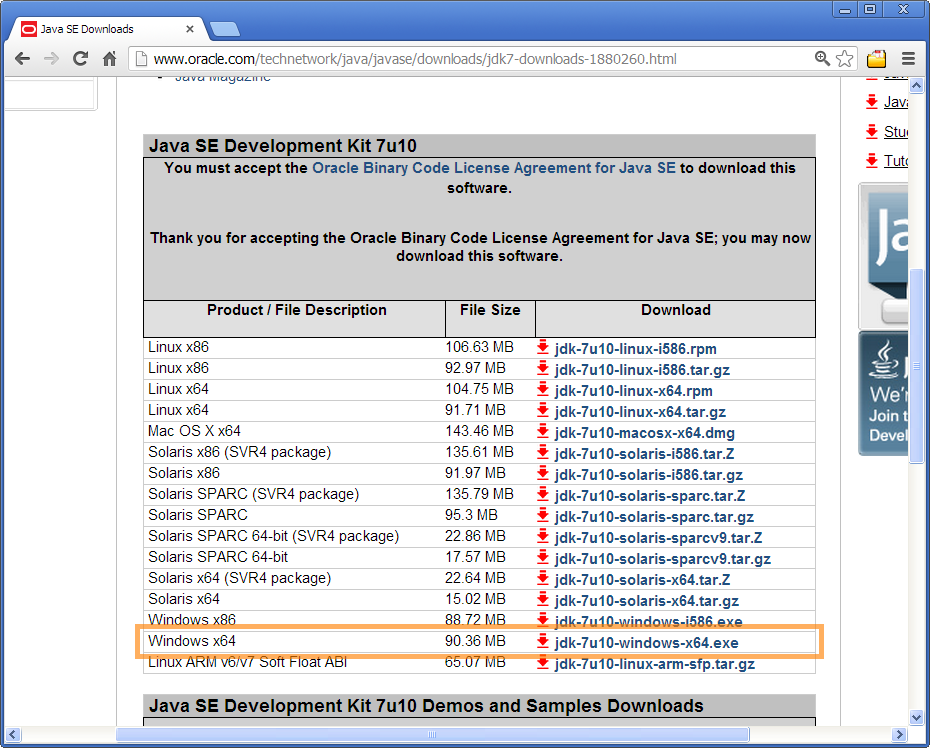
\includegraphics[width=15cm]{oracle_jdk_download.png}
\caption{Installer download for Oracle JDK 7. The Windows 64bit installer package is highlighted.}
\figlabel{jdk_download_oracle}
\end{figure}

Once you have successfully downloaded the JDK installer, follow the Windows installation guide\footnote{
Install the JDK on Windows: \url{http://docs.oracle.com/javase/7/docs/webnotes/install/windows/jdk-installation-windows.html\#Run}}.
To verify the installation you might want to go through this Java ''Hello World!'' 
tutorial\footnote{Windows Java ''Hello World!'': \url{http://docs.oracle.com/javase/tutorial/getStarted/cupojava/win32.html}}.

Installation instructions for Linux\footnote{
Install the JDK on Linux: \url{http://docs.oracle.com/javase/7/docs/webnotes/install/linux/linux-jdk.html}
}
and Mac\footnote{
Install the JDK on Mac: \url{http://docs.oracle.com/javase/7/docs/webnotes/install/mac/mac-jdk.html}.
}
are also available from Oracle.

% --------------------------------------------------------------------------- %
\section{Download and Install Scout}
\seclabel{download_install}

% =========================================================================== %
% TeX input file: "download and install scout"
%
% WARNING: this tex file does not compile standalone, it needs to be embedded
% in a master tex document (e.g. ScoutInstallation.tex)
% =========================================================================== %

Before you can install Scout make sure that you have a working Java Development Kit (JDK) installation of version 7 or 8.
To download the Eclipse Scout package visit the official Eclipse download page as shown in \figref{scout_download}.

\begin{figure}
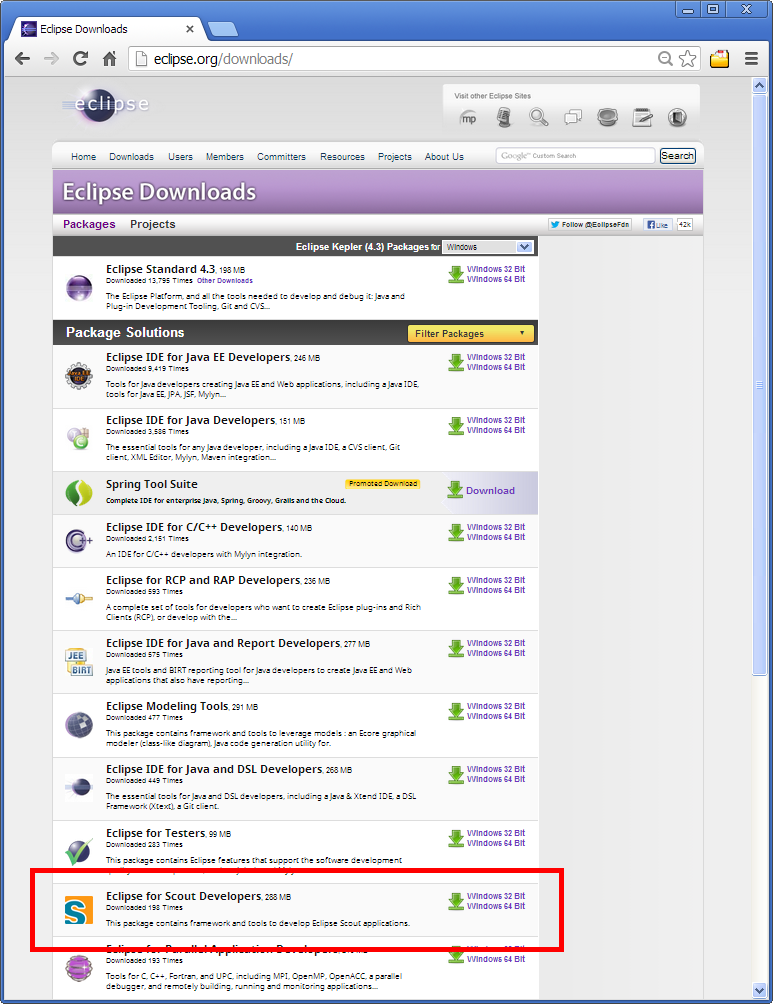
\includegraphics[width=15cm]{scout_download.png}
\caption{The Eclipse download page. The platform filter is set to Windows and the available Packages are filtered for Scout.}
\figlabel{scout_download}
\end{figure}

If the download page shows the wrong platform, manually select the correct platform in the dropdown list.
As shown in \figref{scout_download}, the Scout package is available as a 32 bit and a 46 bit package. 
Make sure to pick the package that matches your JDK installation. 
You can check your installation on the command line as follows.

\begin{lstlisting}[
  language=console
]
console-prompt>java -version
java version "1.7.0_55"
Java(TM) SE Runtime Environment (build 1.7.0_55-b13)
Java HotSpot(TM) 64-Bit Server VM (build 24.55-b03, mixed mode)
\end{lstlisting}

If the output explicitly mentions the 64 bit installation as shown above, you have a 64 bit installation. 
Otherwise, you have a 32 bit JDK installed.
Now you can select the correct Scout package from the Eclipse download site. 
After the package selection, confirm the suggested download mirror as shown in \figref{scout_download_mirror}.

\begin{figure}
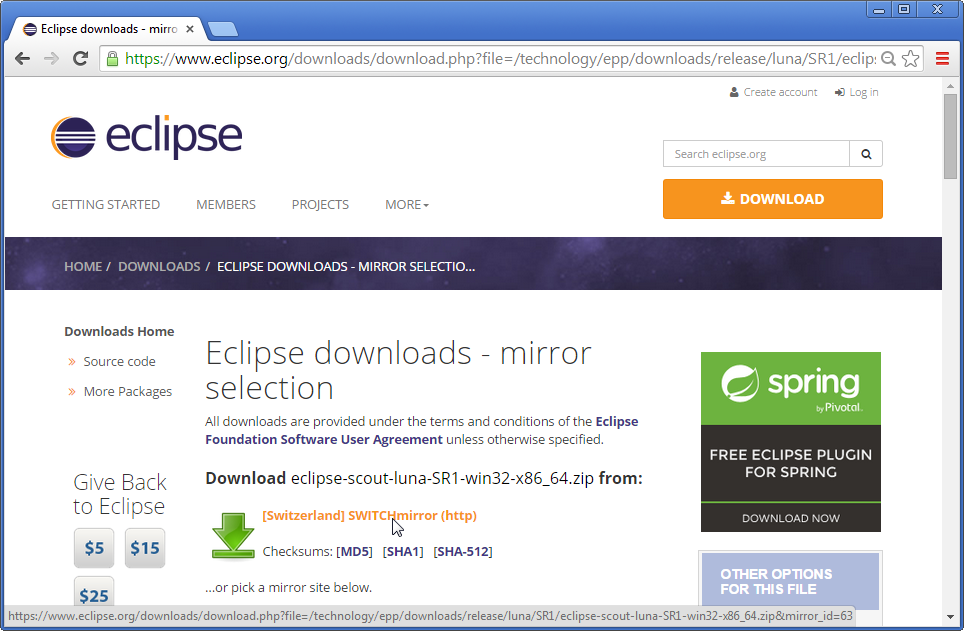
\includegraphics[width=15cm]{scout_download_mirror.png}
\caption{Downloading the Scout package from a mirror.}
\figlabel{scout_download_mirror}
\end{figure}

As the Scout package is a simple ZIP (or tar.gz) file, you may unpack its content to a folder of your choice.
Inside the eclipse sub-folder, you will then find the Eclipse executable file, such as the \texttt{eclipse.exe} file on a Windows plattform. 
Starting the Eclipse executable brings up the workspace launcher as shown in \figref{scout_start}.

\begin{figure}
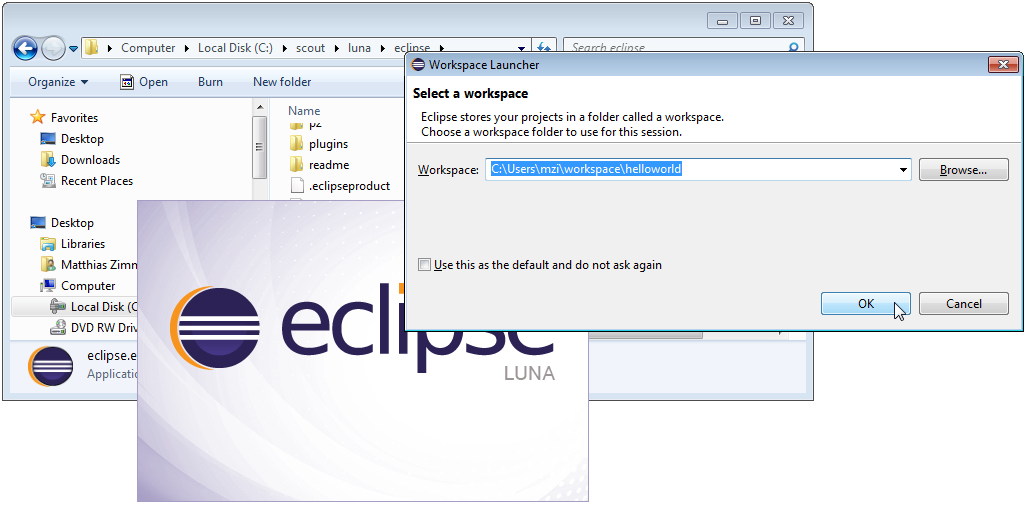
\includegraphics[width=15cm]{scout_startup_select_workspace.png}
\caption{Starting the Eclipse Scout package and selecting an empty workspace.}
\figlabel{scout_start}
\end{figure}

Into the \field{Workspace} you enter an empty target directory for your first Scout project. 
After clicking the \button{Ok}, the Eclipse IDE creates any directories that do not yet exist and opens the specified workspace. 
When opening a new workspace for the first time, Eclipse then displays the welcome screen shown in \figref{scout_welcome}. 

\begin{figure}
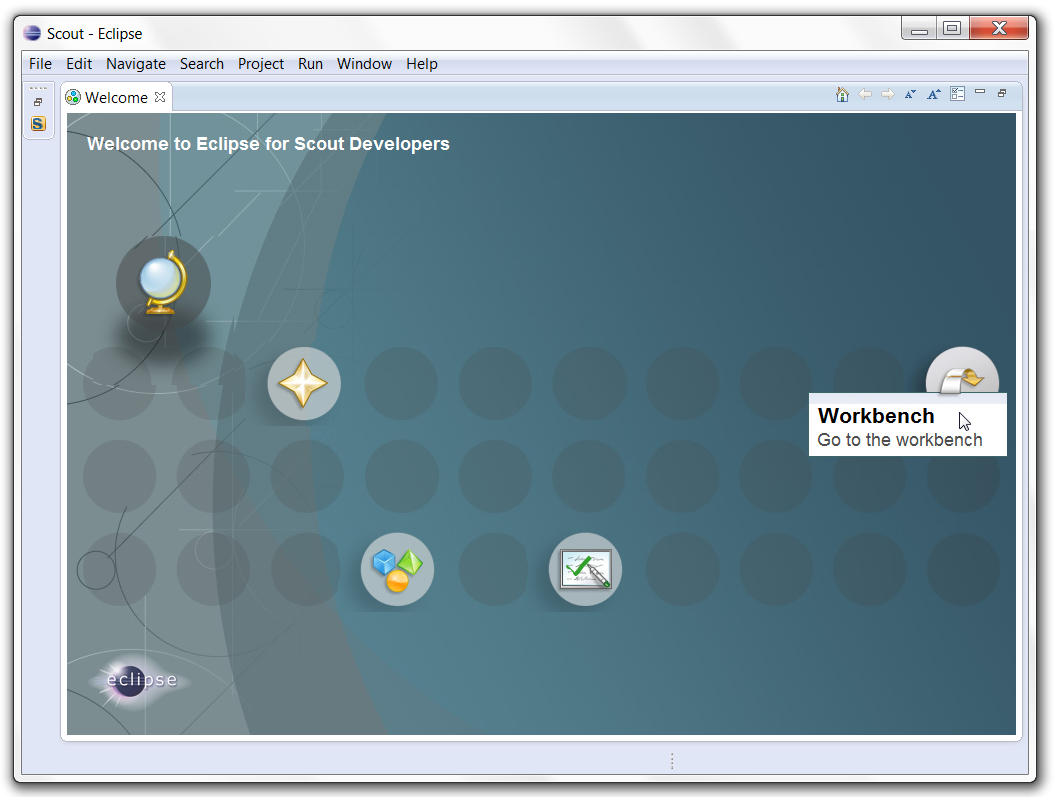
\includegraphics[width=13cm]{scout_startup_welcome.png}
\caption{Eclipse Scout welcome screen.}
\figlabel{scout_welcome}
\end{figure}

To close the welcome page and open the Scout perspective in the Eclipse IDE click on the \icon{Workbench}. 
As a result the empty Scout perspective is displayed according to \figref{scout_perspective}. 

\begin{figure}
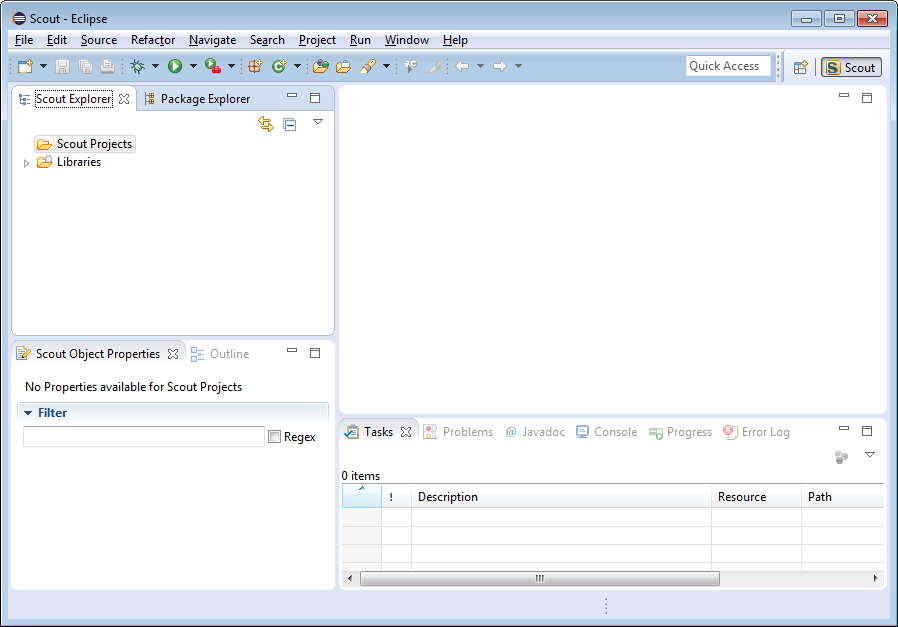
\includegraphics[width=13cm]{scout_startup_scout_explorer.png}
\caption{Eclipse Scout started in the Scout SDK perspective. }
\figlabel{scout_perspective}
\end{figure}

Congratulations, you just have successfully completed the Eclipse Scout installation!

% =========================================================================== %
% EOF TeX input file
% =========================================================================== %


If you have only installed a single JDK you will not need to change the default \texttt{eclipse.ini} file of your Eclipse installation.
In case you have installed multiple JDKs coming with their individual Java Runtime Environments (JREs), you might want to explicitly specifiy which JRE to use.
Open the file \texttt{eclipse.ini} in a editor of your choice and insert the following two lines at the top of the file:

\begin{lstlisting}[
  language=ini
]
-vm
C:\java\jre7\bin\javaw.exe
\end{lstlisting}

where the second line specifies the exact path to the JRE to be used to start your Eclipse Scout installation.

If you have explicitly specified the JRE to be used you verify this in the running Eclipse installation.
Fist, select the \menu{Help|About Eclipse} to open the about dialog.
Then, click on the \button{Installation Details} and switch to the \tab{Configuration}.
In the long list of system properties you will find lines similar to the ones shown below.

\begin{lstlisting}[
  language=ini
]
*** Date: Donnerstag, 19. Juni 2014 10:37:17 Normalzeit

*** Platform Details:

*** System properties:
...
-vm
C:\java\jre7\bin\javaw.exe
...
sun.java.command=... vm C:\java\jre7\bin\javaw.exe -vmargs ...
\end{lstlisting}

You have now successfully completed the Eclipse Scout installation on your Windows environment.
With this running Scout installation you may skip the following section on how to add Scout to an existing Eclipse installation.

% --------------------------------------------------------------------------- %
\section{Add Scout to your Eclipse Installation}

This section describes the installation of Scout into an existing Eclipse installation.
As the audience of this section is assumed to be familiar with Eclipse, we do not describe how you got your Eclipse installation in the first place.
For the provided screenshots we start from the popular package \textit{Eclipse IDE for Java EE Developers}.

\begin{figure}
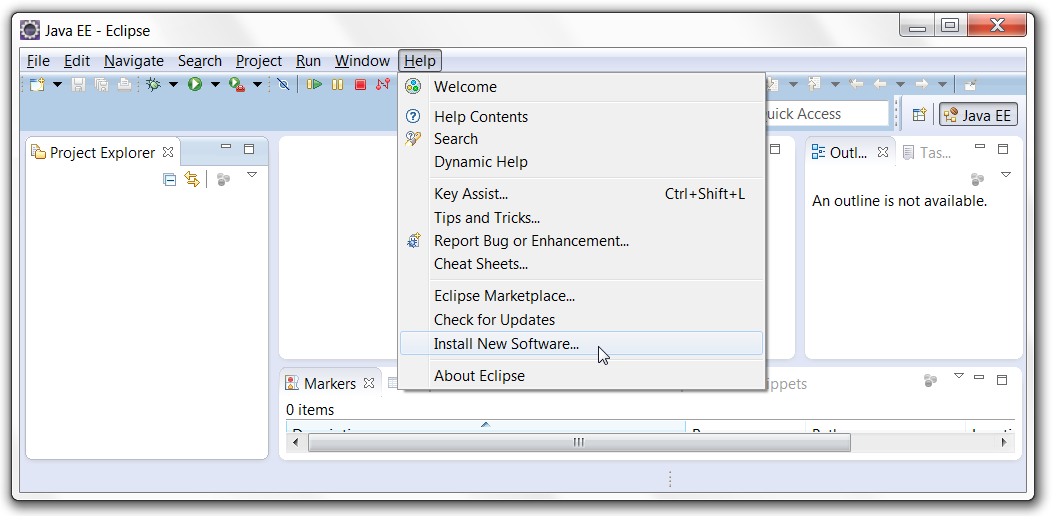
\includegraphics[width=13cm]{eclipse_install_new_software.png}
\caption{Eclipse menu to install additional software}
\figlabel{eclipse_install_new_software}
\end{figure}

To add Scout to your existing Eclipse installation, you need to start Eclipse.
Then select the \menu{Help|Install New Software...} as shown in \figref{eclipse_install_new_software} to open the install dialog.

\begin{figure}
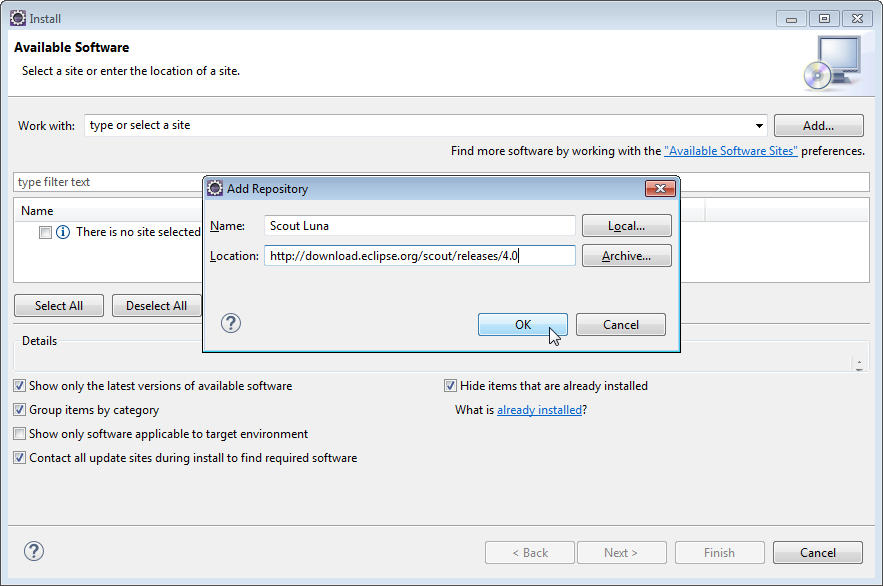
\includegraphics[width=13cm]{eclipse_add_repository.png}
\caption{Add the current Scout repository}
\figlabel{eclipse_add_repository}
\end{figure}

In the install dialog, click on the \button{Add...} to enter the link to the Scout repository.
This opens the popup dialog \textit{Add Repository}
As shown in \figref{eclipse_add_repository}, you may use ''Scout Luna'' for the \field{Name}.
For the \field{Location} enter the Scout release repository as specified below.
\url{http://download.eclipse.org/scout/releases/4.0}.

\begin{figure}
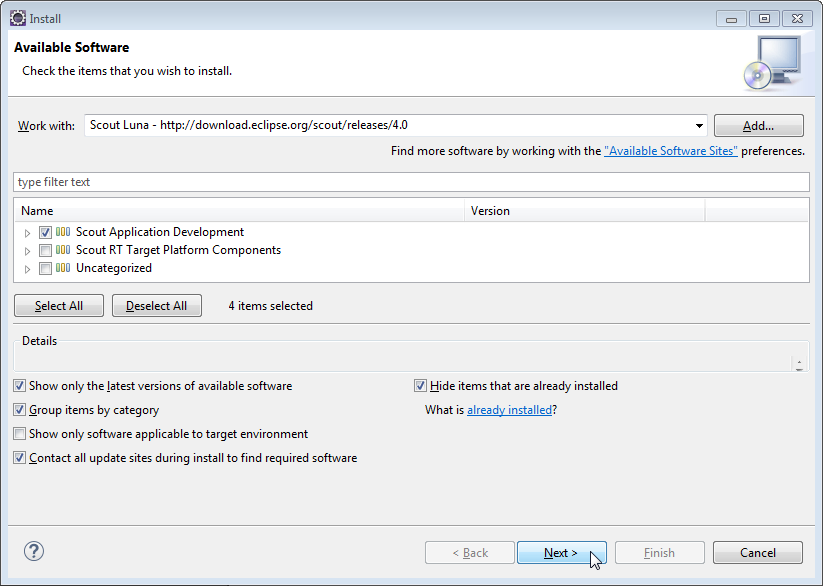
\includegraphics[width=13cm]{eclipse_select_scout_features.png}
\caption{Select the Scout features to add to the Eclipse installation}
\figlabel{eclipse_select_scout_features}
\end{figure}

After the Eclipse IDE has connected to the Scout repository, select the Scout feature \textit{Scout Application Development} as shown in \figref{eclipse_select_scout_features}.
Then, move through the installation with the \button{Next}.
On the last installation step, accept the presented EPL terms by clicking on the appropriate radio button. 
To complete the installation, click the \button{Finish} and accept the request for a restart of Eclipse.
After the restart of the Eclipse IDE, you may add the Scout perspective using the \menu{Window|Open Perspective|Other ...} and selecting the Scout perspective from the presented list. 
Clicking on the Scout perspective button should then result in a state very similar to \figref{scout_perspective}.

% --------------------------------------------------------------------------- %
\section{Verifying the Installation}

After you can start your Eclipse Scout package you need to verify that Scout is working as intended.
The simplest way to verify your Scout installation is to create a ''Hello World'' Scout project and run the corresponding Scout application as described in \charef{helloworld}.

% =========================================================================== %
\chapter{Apache Tomcat Installation}
\applabel{install_tomcat}

Apache Tomcat is an open source web server that is a widely used implementation of the Java Servlet Specification.
Specifically, Tomcat works very well to run the server part of Scout client server applications.
In case you are interested in getting some general context around Tomcat you could start with the Wikipedia article\footnote{
Apache Tomcat Wikipedia: \url{http://en.wikipedia.org/wiki/Apache_Tomcat}.
}.
Then get introduced to its core component ''Tomcat Catalina''\footnote{
Mulesoft's introduction to Tomcat Catalina: \url{http://www.mulesoft.com/tomcat-catalina}.
}
before you switch to the official Tomcat homepage\footnote{
Apache Tomcat Homepage: \url{http://tomcat.apache.org/}
}.

This section is not really a step by step download and installation guide. 
Rather, it points you to the proper places for downloading and installing Tomcat.
We recommend to work with Tomcat version 7.0.
Start your download from the official download site\footnote{
Tomcat 7 Downloads: \url{http://tomcat.apache.org/download-70.cgi}
}.

\begin{figure}
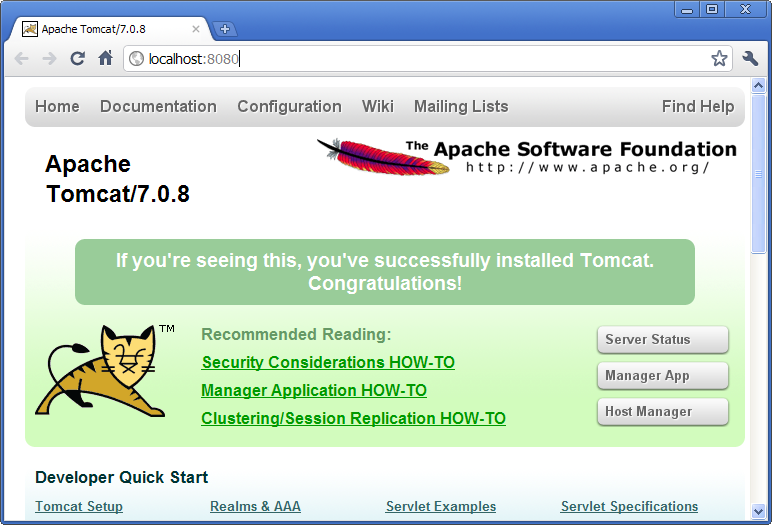
\includegraphics[width=14cm]{tomcat_install.png}
\caption{A successful Tomcat 7 installation.}
\figlabel{tomcat_install}
\end{figure}

Once you have downloaded and installed Tomcat 7 (see the sections below for plattform specific guidelines) you can start the corresponding service or deamon.
To verify that Tomcat is actually running open a web browser of your choice and type \url{http://localhost:8080} into the address bar.
You should then see a confirmation of the successful installation according to \figref{tomcat_install}.

% ........................................................................... %
\section{Platform Specific Instructions}

According to the Tomcat setup installation for Windows\footnote{
Tomcat Windows setup: \url{http://tomcat.apache.org/tomcat-7.0-doc/setup.html#Windows}
}
download the package ''32-bit/64-bit Windows Service Installer'' from the \href{http://tomcat.apache.org/download-70.cgi}{Tomcat 7 download site}.
Then, start the installer and accept the proposed default settings.

For installing Tomcat on OS X systems download the ''tar.gz'' package from the \href{http://tomcat.apache.org/download-70.cgi}{Tomcat 7 download site}.
Then, follow the installation guide\footnote{
Installing Tomcat on OS X: \url{http://wolfpaulus.com/journal/mac/tomcat7}
} provided by Wolf Paulus.

For Linux systems download the ''tar.gz'' package from the \href{http://tomcat.apache.org/download-70.cgi}{Tomcat 7 download site}.
Then, follow the description of the Unix setup\footnote{
Tomcat Linux setup: \url{http://tomcat.apache.org/tomcat-7.0-doc/setup.html#Unix_daemon}
}
to run Tomcat as a deamon.
If you use Ubuntu, you may want to follow the tutorial\footnote{
Apache Tomcat Tutorial: \url{http://www.vogella.com/articles/ApacheTomcat/article.html}
} 
for downloading and installing Tomcat provided by Lars Vogel.


% ........................................................................... %
\section{Directories and Files}
\applabel{tomcat_dirs_and_files}

Tomcat's installation directory follows the same organisation on all platforms.
Here, we will only introduce the most important aspects of the Tomcat installation for the purpose of this book.

\begin{figure}
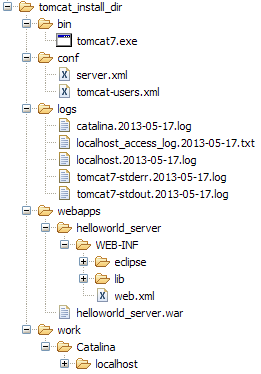
\includegraphics[width=6cm]{tomcat_install_dir.png}
\caption{The organisation of a Tomcat installation including specific files of interest.
As an example, the ''Hello World'' server application is contained in subdirectory \texttt{webapps}.
}
\figlabel{tomcat_install_dir}
\end{figure}

Note that some folders and many files of a Tomcat installation are not represented in \figref{tomcat_install_dir}.
We just want to provide a basic understanding of the most important parts to operate the web server in the context of this book.
In the \filename{bin} folder, the executable programs are contained, including scripts to start and stop the Tomcat instance.

The \filename{conf} folder contains a set of XML and property configuration file.
The file \filename{server.xml} represents Tomcat's main configuration file.
It is used to configure general web server aspects such as the port number of its connectors for the client server communication.
For the default setup, port number 8080 is used for the communication between clients applications and the web server.
The file \filename{tomcat-users.xml} contains a database of users, passwords and associated roles.

Folder \filename{logs} contains various logfiles of Tomcat itself as well as host and web application log files.
XXX need to provide more on what is where (especially application logs and exact setup to generate log entries from scout apps).

The folder needed for deploying web applications into a Tomcat instance is called \filename{webapps}.
It can be used as the target for copying WAR files into the web server.
The installation of the WAR file then extracts its content into the corresponding directory structure as shown in \figref{tomcat_install_dir} in the case of the file \filename{helloworld_server.war}.

Finally, folder \filename{work} contains Tomcat's runtime ''cache'' for the deployed web applications.
It is organized according to the hierarchy of the engine (Catalina), the host (localhost), and the web application (\filename{helloworld_server}).

% ........................................................................... %
\section{The Tomcat Manager Application}
\applabel{tomcat_manager_app}

Tomcat comes with the pre installed ''Manager App''.
This application is useful to manage web applications and perform tasks such as deploying a web application from a WAR file, or starting and stopping installed web applications.
A comprehensive documentation for the ''Manager App'' can be found under the Tomcat homepage\footnote{
The Tomcat Manager Application: \url{http://tomcat.apache.org/tomcat-7.0-doc/manager-howto.html}.
}.
Here we only show how to start this application from the hompage of a running Tomcat installation.

To access this application you can switch to the ''Manager App'' with a click on the corresponding button on the right hand side.
The button can be found on the right hand side of \figref{tomcat_install}.
Before you are allowed to start this application, you need to provide username and password credentials of a user associated with Tomcats's \java{manager-gui} role.

\begin{lstlisting}[
  language=xml,
  float,
  label=\lstlabel{tomcat.users},
  caption=Example content for a \texttt{tomcat-users.xml} file]
  <tomcat-users>
    <!--
    NOTE: By default, no user is included in the "manager-gui" role required
    to operate the "/manager/html" web application. If you wish to use it
    you must define such a user - the username and password are arbitrary.
    -->
	<user name="admin" password="s3cret" roles="manager-gui"/>
  </tomcat-users>	
\end{lstlisting}

To get at user names and passwords you can open file \filename{tomcat-users.xml} located in Tomcat's \filename{conf} directory.
In this file the active users with their passwords and associated roles are stored.
See \lstref{tomcat.users} for an example.
From the content of this file, we see that user \java{admin} has password \java{s3cret} and also posesses the necessary role \java{manager-gui} to access the ''Manager App''.
If file \filename{tomcat-users.xml} does not contain any user with this role, you can simply add new user with this role to the existing users.
Alternatively, you also can add the necessary role to an existing user.
Just append a comma to the existing right(s) followed by the string \java{manager-gui}.
Note that you will need to restart your Tomcat application after adapting the content of file \filename{tomcat-users.xml}.

With working credentials you can now start the ''Manager App'' as described the ''Hello World'' tutorial in \secref{helloworld_deploy}.

% --------------------------------------------------------------------------- %

\ifx\wholebook\relax\else
   \begin{thebibliography}{99}
  \addcontentsline{toc}{chapter}{Bibliography}
  
  % add/insert books in alphabetical order of 1st author
  
  \bibitem{batessierra05}
    \textit{Bert Bates, Kathy Sierra},
	\textbf{Head First Java} 2nd edition, 
	O'Reilly Media, 2005.

  \bibitem{bloch08} 
    \textit{Joshua Bloch},
    \textbf{Effective Java} 2nd edition, 
	Addison-Wesley, 2008.
	
  \bibitem{eckel06}
    \textit{Bruce Eckel},
	\textbf{Thinking in Java} 4th edition, 
	Prentice Hall International, 2006.

\end{thebibliography}

   \end{document}
\fi

% =========================================================================== %

% =========================================================================== %
% Useful Utilities
% =========================================================================== %

\ifx\wholebook\relax\else
  \documentclass[a4paper,10pt,twoside]{book}
  %=============================================================================%
% Common things, settings, packages to include
%=============================================================================%

\usepackage{graphicx}
\usepackage{color}
\usepackage{makeidx}
\usepackage{ifpdf}
\usepackage{verbatim}

% --------------------------------------------------------------------------- %
% Setting up stuff depeding on output format
% --------------------------------------------------------------------------- %

\ifpdf
  % special settings for pdf mode
  \usepackage[colorlinks]{hyperref}
  \usepackage{courier}
  
  \hypersetup{
    colorlinks,
    linkcolor=darkblue,
    citecolor=darkblue,
    pdftitle={The Eclipse Scout Book},
    pdfauthor={The Scout Community},
    pdfkeywords={Enterprise Framework, Eclipse, Java, Client-Side, Rich Client, Web Client, Mobile},
    pdfsubject={Computer Science}
  }
  
  \usepackage{caption}
  \captionsetup{margin=10pt,font=small,labelfont=bf}
\else
  % special stuff for html mode
  \usepackage[tex4ht]{hyperref}
\fi

% --------------------------------------------------------------------------- %
% Setting up printing range
% --------------------------------------------------------------------------- %

\parindent 1cm
\parskip 0.2cm
\topmargin 0.2cm
\oddsidemargin 1cm
\evensidemargin 0.5cm
\textwidth 15cm
\textheight 21cm

% --------------------------------------------------------------------------- %
% Setting up listings
% --------------------------------------------------------------------------- %

\usepackage{listings}
 
\definecolor{darkviolet}{rgb}{0.5,0,0.4}
\definecolor{darkgreen}{rgb}{0,0.4,0.2} 
\definecolor{darkblue}{rgb}{0.1,0.1,0.9}
\definecolor{darkgrey}{rgb}{0.5,0.5,0.5}
\definecolor{lightblue}{rgb}{0.4,0.4,1}
\definecolor{lightgray}{rgb}{0.97,0.97,0.97}

\renewcommand{\lstlistlistingname}{List of Listings}

% general settings
\lstset{
  basicstyle=\small\ttfamily,
  columns=fullflexible,
  breaklines=true,
  breakindent=10pt,
  prebreak=\mbox{{\color{blue}\tiny$\searrow$}},
  postbreak=\mbox{{\color{blue}\tiny$\rightarrow$}},
  showstringspaces=false,
  backgroundcolor=\color{lightgray}
}

% settings for xml files
\lstdefinelanguage{xml}
{
  commentstyle=\color{darkgrey}\upshape,
  morestring=[b]",
  morestring=[s]{>}{<},
  morecomment=[s]{<?}{?>},
  stringstyle=\color{black},
  identifierstyle=\color{darkblue},
  keywordstyle=\color{cyan},
  morekeywords={xmlns,name,point,factory,class}% list your attributes here
}

% settings for ini files
\lstdefinelanguage{ini}
{
  morecomment=[f][\color{darkgrey}\upshape][0]\#, % # is comment iff it's the first char on the line
  stringstyle=\color{black}
}

% default settings (for java files)
\lstset{
  language=Java,
  emphstyle=\color{red}\bfseries,
  keywordstyle=\color{darkviolet}\bfseries,
  commentstyle=\color{darkgreen},
  morecomment=[s][\color{lightblue}]{/**}{*/},
  stringstyle=\color{darkblue},
}

% --------------------------------------------------------------------------- %
% cross reference macros
% --------------------------------------------------------------------------- %
\newcommand{\applabel}[1]{\label{apx:#1}}
\newcommand{\chalabel}[1]{\label{cha:#1}}
\newcommand{\seclabel}[1]{\label{sec:#1}}
\newcommand{\lstlabel}[1]{\label{lst:#1}}
\newcommand{\figlabel}[1]{\label{fig:#1}}
\newcommand{\tablabel}[1]{\label{tab:#1}}

\newcommand{\appref}[1]{Appendix~\ref{apx:#1}}
\newcommand{\charef}[1]{Chapter~\ref{cha:#1}\xspace}
\newcommand{\secref}[1]{Section~\ref{sec:#1}}
\newcommand{\lstref}[1]{Listing~\ref{lst:#1}\xspace}
\newcommand{\figref}[1]{Figure~\ref{fig:#1}\xspace}
\newcommand{\tabref}[1]{Table~\ref{tab:#1}\xspace}

% --------------------------------------------------------------------------- %
% graphics paths
% --------------------------------------------------------------------------- %
\graphicspath{
  {figures/}
  {Introduction/figures/}
}

%=============================================================================%

  \pagestyle{headings}
  \graphicspath{{figures/} {../figures/}}
  \begin{document}
  \sloppy
\fi


% --------------------------------------------------------------------------- %
\chapter{Useful Scout Utility Classes}
text needed

1) <ctrl-shift-t>fileutility
2) click into package org.eclipse.scout.commons;
3) <alt-shift-w> (or context menu) show-in package explorer

% --------------------------------------------------------------------------- %
\section{StringUtility}
text needed


% --------------------------------------------------------------------------- %
\section{DateUtility}
text needed


% --------------------------------------------------------------------------- %
\section{FileUtility}
text needed

\noindent Existing Documentation
\begin{itemize}
  \item bug \url{https://bugs.eclipse.org/bugs/show_bug.cgi?id=394784}
\end{itemize}

% --------------------------------------------------------------------------- %

\ifx\wholebook\relax\else
   \begin{thebibliography}{99}
  \addcontentsline{toc}{chapter}{Bibliography}
  
  % add/insert books in alphabetical order of 1st author
  
  \bibitem{batessierra05}
    \textit{Bert Bates, Kathy Sierra},
	\textbf{Head First Java} 2nd edition, 
	O'Reilly Media, 2005.

  \bibitem{bloch08} 
    \textit{Joshua Bloch},
    \textbf{Effective Java} 2nd edition, 
	Addison-Wesley, 2008.
	
  \bibitem{eckel06}
    \textit{Bruce Eckel},
	\textbf{Thinking in Java} 4th edition, 
	Prentice Hall International, 2006.

\end{thebibliography}

   \end{document}
\fi

% =========================================================================== %

% =========================================================================== %
% Java Basics
% =========================================================================== %

\ifx\wholebook\relax\else
  \documentclass[a4paper,10pt,twoside]{book}
  %=============================================================================%
% Common things, settings, packages to include
%=============================================================================%

\usepackage{graphicx}
\usepackage{color}
\usepackage{makeidx}
\usepackage{ifpdf}
\usepackage{verbatim}

% --------------------------------------------------------------------------- %
% Setting up stuff depeding on output format
% --------------------------------------------------------------------------- %

\ifpdf
  % special settings for pdf mode
  \usepackage[colorlinks]{hyperref}
  \usepackage{courier}
  
  \hypersetup{
    colorlinks,
    linkcolor=darkblue,
    citecolor=darkblue,
    pdftitle={The Eclipse Scout Book},
    pdfauthor={The Scout Community},
    pdfkeywords={Enterprise Framework, Eclipse, Java, Client-Side, Rich Client, Web Client, Mobile},
    pdfsubject={Computer Science}
  }
  
  \usepackage{caption}
  \captionsetup{margin=10pt,font=small,labelfont=bf}
\else
  % special stuff for html mode
  \usepackage[tex4ht]{hyperref}
\fi

% --------------------------------------------------------------------------- %
% Setting up printing range
% --------------------------------------------------------------------------- %

\parindent 1cm
\parskip 0.2cm
\topmargin 0.2cm
\oddsidemargin 1cm
\evensidemargin 0.5cm
\textwidth 15cm
\textheight 21cm

% --------------------------------------------------------------------------- %
% Setting up listings
% --------------------------------------------------------------------------- %

\usepackage{listings}
 
\definecolor{darkviolet}{rgb}{0.5,0,0.4}
\definecolor{darkgreen}{rgb}{0,0.4,0.2} 
\definecolor{darkblue}{rgb}{0.1,0.1,0.9}
\definecolor{darkgrey}{rgb}{0.5,0.5,0.5}
\definecolor{lightblue}{rgb}{0.4,0.4,1}
\definecolor{lightgray}{rgb}{0.97,0.97,0.97}

\renewcommand{\lstlistlistingname}{List of Listings}

% general settings
\lstset{
  basicstyle=\small\ttfamily,
  columns=fullflexible,
  breaklines=true,
  breakindent=10pt,
  prebreak=\mbox{{\color{blue}\tiny$\searrow$}},
  postbreak=\mbox{{\color{blue}\tiny$\rightarrow$}},
  showstringspaces=false,
  backgroundcolor=\color{lightgray}
}

% settings for xml files
\lstdefinelanguage{xml}
{
  commentstyle=\color{darkgrey}\upshape,
  morestring=[b]",
  morestring=[s]{>}{<},
  morecomment=[s]{<?}{?>},
  stringstyle=\color{black},
  identifierstyle=\color{darkblue},
  keywordstyle=\color{cyan},
  morekeywords={xmlns,name,point,factory,class}% list your attributes here
}

% settings for ini files
\lstdefinelanguage{ini}
{
  morecomment=[f][\color{darkgrey}\upshape][0]\#, % # is comment iff it's the first char on the line
  stringstyle=\color{black}
}

% default settings (for java files)
\lstset{
  language=Java,
  emphstyle=\color{red}\bfseries,
  keywordstyle=\color{darkviolet}\bfseries,
  commentstyle=\color{darkgreen},
  morecomment=[s][\color{lightblue}]{/**}{*/},
  stringstyle=\color{darkblue},
}

% --------------------------------------------------------------------------- %
% cross reference macros
% --------------------------------------------------------------------------- %
\newcommand{\applabel}[1]{\label{apx:#1}}
\newcommand{\chalabel}[1]{\label{cha:#1}}
\newcommand{\seclabel}[1]{\label{sec:#1}}
\newcommand{\lstlabel}[1]{\label{lst:#1}}
\newcommand{\figlabel}[1]{\label{fig:#1}}
\newcommand{\tablabel}[1]{\label{tab:#1}}

\newcommand{\appref}[1]{Appendix~\ref{apx:#1}}
\newcommand{\charef}[1]{Chapter~\ref{cha:#1}\xspace}
\newcommand{\secref}[1]{Section~\ref{sec:#1}}
\newcommand{\lstref}[1]{Listing~\ref{lst:#1}\xspace}
\newcommand{\figref}[1]{Figure~\ref{fig:#1}\xspace}
\newcommand{\tabref}[1]{Table~\ref{tab:#1}\xspace}

% --------------------------------------------------------------------------- %
% graphics paths
% --------------------------------------------------------------------------- %
\graphicspath{
  {figures/}
  {Introduction/figures/}
}

%=============================================================================%

  \pagestyle{headings}
  \graphicspath{{figures/} {../figures/}}
  \begin{document}
  \sloppy
\fi


% --------------------------------------------------------------------------- %
\chapter{Java Basics}
\applabel{java_basics}

% --------------------------------------------------------------------------- %
\section{Java SE Basics}
\applabel{javase_basics}

\fbox{
  \parbox{12cm}{
    Section waiting for contribution (2'000-3'000 words)
	
    The goal of this section is to provide the reader with a solid overview of the non-trivial
    Java concepts relevant for scout applications and central aspects of the framework itself.
    The focus of this section is on the Java Standard Edition (Java SE).
    Where appropriate, provide links to high quality online material, that is likely to exist for at least the next year or two.
  }
}

\subsection{Learning Java}

To progam Scout applications you need to have a solid understanding of the Java language.
Scout will only work for you if you have achieved a certain proficiency level in Java. 

Luckily, free online tutorials to learn Java are offered in many places.
A good starting point is the official Java documentation 
site\footnote{Official online Java tutorial: \url{http://docs.oracle.com/javase/tutorial/}}.
If you prefer to work with video tutorials we recommend ``Eclipse and Java for Total 
Beginners''\footnote{Eclipse and Java for Total Beginners: \url{http://eclipsetutorial.sourceforge.net/totalbeginner.html}}, 
although the installation used is somewhat out of date.
As for printed books, we suggest to start with either ``Head First Java''\cite{batessierra05} or ``Thinking in Java''\cite{eckel06}.
Highly recommended but slightly more advanced is ``Effective Java''\cite{bloch08}.

To solve really tricky Java problems there is often no way around the Java 
specification\footnote{The Java Language Specification \url{http://docs.oracle.com/javase/specs/}} itself.
Just make sure to pick the right Java version for your context.

\subsection{Advanced Java SE Concepts}

  * say which non-trivial things are vital to good understanding
  * threading
  * generics
  * annotations

% --------------------------------------------------------------------------- %
\section{Java EE Basics}
\applabel{javaee_basics}

\fbox{
  \parbox{12cm}{
    Section waiting for contribution (2'000-5'000 words)
    
    The goal of this section is to provide the reader with a solid overview of the non-trivial
    Java enterprise concepts relevant for scout applications and central aspects of the framework itself. 
	The focus of this section is on the Java Enterprise Edition (Java EE)
    Where appropriate, provide links to high quality online material, that is likely to exist for at least the next year or two.
  }
}

needs text

  * maybe the same as for java foundation, maybe not
  * jaas
  * http comm
  * servlet
  * servlet filters


\lstinputlisting[
  label=\lstlabel{tinyservlet.web_xml},
  caption=The \java{index.html} start page for the tiny servlet application.,
  language=html,
  float
]
{../code/tinyservlet/index.html}

\lstinputlisting[
  label=\lstlabel{tinyservlet.web_xml},
  caption=The \java{web.xml} file of the tiny servlet application.,
  language=xml,
  float
]
{../code/tinyservlet/WEB-INF/web.xml}

\lstinputlisting[
  label=\lstlabel{tinyservlet.TinyServlet},
  caption=The complete \java{TinyServlet} source code.,
  float
]
{../code/tinyservlet/WEB-INF/sources/TinyServlet.java}

war file organisation: \url{http://documentation.progress.com/output/Iona/orbix/6.1/tutorials/fnb/dev_intro/j2ee_overview8.html}

% --------------------------------------------------------------------------- %

\ifx\wholebook\relax\else
   \begin{thebibliography}{99}
  \addcontentsline{toc}{chapter}{Bibliography}
  
  % add/insert books in alphabetical order of 1st author
  
  \bibitem{batessierra05}
    \textit{Bert Bates, Kathy Sierra},
	\textbf{Head First Java} 2nd edition, 
	O'Reilly Media, 2005.

  \bibitem{bloch08} 
    \textit{Joshua Bloch},
    \textbf{Effective Java} 2nd edition, 
	Addison-Wesley, 2008.
	
  \bibitem{eckel06}
    \textit{Bruce Eckel},
	\textbf{Thinking in Java} 4th edition, 
	Prentice Hall International, 2006.

\end{thebibliography}

   \end{document}
\fi

% =========================================================================== %

% =========================================================================== %
% Eclipse Basics
% =========================================================================== %

\ifx\wholebook\relax\else
  \documentclass[a4paper,10pt,twoside]{book}
  %=============================================================================%
% Common things, settings, packages to include
%=============================================================================%

\usepackage{graphicx}
\usepackage{color}
\usepackage{makeidx}
\usepackage{ifpdf}
\usepackage{verbatim}

% --------------------------------------------------------------------------- %
% Setting up stuff depeding on output format
% --------------------------------------------------------------------------- %

\ifpdf
  % special settings for pdf mode
  \usepackage[colorlinks]{hyperref}
  \usepackage{courier}
  
  \hypersetup{
    colorlinks,
    linkcolor=darkblue,
    citecolor=darkblue,
    pdftitle={The Eclipse Scout Book},
    pdfauthor={The Scout Community},
    pdfkeywords={Enterprise Framework, Eclipse, Java, Client-Side, Rich Client, Web Client, Mobile},
    pdfsubject={Computer Science}
  }
  
  \usepackage{caption}
  \captionsetup{margin=10pt,font=small,labelfont=bf}
\else
  % special stuff for html mode
  \usepackage[tex4ht]{hyperref}
\fi

% --------------------------------------------------------------------------- %
% Setting up printing range
% --------------------------------------------------------------------------- %

\parindent 1cm
\parskip 0.2cm
\topmargin 0.2cm
\oddsidemargin 1cm
\evensidemargin 0.5cm
\textwidth 15cm
\textheight 21cm

% --------------------------------------------------------------------------- %
% Setting up listings
% --------------------------------------------------------------------------- %

\usepackage{listings}
 
\definecolor{darkviolet}{rgb}{0.5,0,0.4}
\definecolor{darkgreen}{rgb}{0,0.4,0.2} 
\definecolor{darkblue}{rgb}{0.1,0.1,0.9}
\definecolor{darkgrey}{rgb}{0.5,0.5,0.5}
\definecolor{lightblue}{rgb}{0.4,0.4,1}
\definecolor{lightgray}{rgb}{0.97,0.97,0.97}

\renewcommand{\lstlistlistingname}{List of Listings}

% general settings
\lstset{
  basicstyle=\small\ttfamily,
  columns=fullflexible,
  breaklines=true,
  breakindent=10pt,
  prebreak=\mbox{{\color{blue}\tiny$\searrow$}},
  postbreak=\mbox{{\color{blue}\tiny$\rightarrow$}},
  showstringspaces=false,
  backgroundcolor=\color{lightgray}
}

% settings for xml files
\lstdefinelanguage{xml}
{
  commentstyle=\color{darkgrey}\upshape,
  morestring=[b]",
  morestring=[s]{>}{<},
  morecomment=[s]{<?}{?>},
  stringstyle=\color{black},
  identifierstyle=\color{darkblue},
  keywordstyle=\color{cyan},
  morekeywords={xmlns,name,point,factory,class}% list your attributes here
}

% settings for ini files
\lstdefinelanguage{ini}
{
  morecomment=[f][\color{darkgrey}\upshape][0]\#, % # is comment iff it's the first char on the line
  stringstyle=\color{black}
}

% default settings (for java files)
\lstset{
  language=Java,
  emphstyle=\color{red}\bfseries,
  keywordstyle=\color{darkviolet}\bfseries,
  commentstyle=\color{darkgreen},
  morecomment=[s][\color{lightblue}]{/**}{*/},
  stringstyle=\color{darkblue},
}

% --------------------------------------------------------------------------- %
% cross reference macros
% --------------------------------------------------------------------------- %
\newcommand{\applabel}[1]{\label{apx:#1}}
\newcommand{\chalabel}[1]{\label{cha:#1}}
\newcommand{\seclabel}[1]{\label{sec:#1}}
\newcommand{\lstlabel}[1]{\label{lst:#1}}
\newcommand{\figlabel}[1]{\label{fig:#1}}
\newcommand{\tablabel}[1]{\label{tab:#1}}

\newcommand{\appref}[1]{Appendix~\ref{apx:#1}}
\newcommand{\charef}[1]{Chapter~\ref{cha:#1}\xspace}
\newcommand{\secref}[1]{Section~\ref{sec:#1}}
\newcommand{\lstref}[1]{Listing~\ref{lst:#1}\xspace}
\newcommand{\figref}[1]{Figure~\ref{fig:#1}\xspace}
\newcommand{\tabref}[1]{Table~\ref{tab:#1}\xspace}

% --------------------------------------------------------------------------- %
% graphics paths
% --------------------------------------------------------------------------- %
\graphicspath{
  {figures/}
  {Introduction/figures/}
}

%=============================================================================%

  \pagestyle{headings}
  \graphicspath{{figures/} {../figures/}}
  \begin{document}
  \sloppy
\fi


% --------------------------------------------------------------------------- %
\chapter{Eclipse Basics}

% --------------------------------------------------------------------------- %
\section{Overview}
needs text

% --------------------------------------------------------------------------- %
\section{OSGi}
needs text

  * bundles
  * services
  
% --------------------------------------------------------------------------- %
\section{Eclipse}
needs text

  * plugins
  * fragments
  * features
  * products
  * targets
  * servlet bridge
  * client exe files
  
% --------------------------------------------------------------------------- %
  
\ifx\wholebook\relax\else
   \begin{thebibliography}{99}
  \addcontentsline{toc}{chapter}{Bibliography}
  
  % add/insert books in alphabetical order of 1st author
  
  \bibitem{batessierra05}
    \textit{Bert Bates, Kathy Sierra},
	\textbf{Head First Java} 2nd edition, 
	O'Reilly Media, 2005.

  \bibitem{bloch08} 
    \textit{Joshua Bloch},
    \textbf{Effective Java} 2nd edition, 
	Addison-Wesley, 2008.
	
  \bibitem{eckel06}
    \textit{Bruce Eckel},
	\textbf{Thinking in Java} 4th edition, 
	Prentice Hall International, 2006.

\end{thebibliography}

   \end{document}
\fi

% =========================================================================== %


% --------------------------------------------------------------------------- %
% Lists of various things
% --------------------------------------------------------------------------- %

\pagestyle{plain}

% lstlistoflistings seems to be broken for tex4ht
% skip complete reference section for html output
\ifpdf
  \listoffigures
  \addcontentsline{toc}{chapter}{Figures}

  \listoftables
  \addcontentsline{toc}{chapter}{Tables}
  
  \lstlistoflistings
  \addcontentsline{toc}{chapter}{Listings}
\fi

% --------------------------------------------------------------------------- %
% Bibliography
% --------------------------------------------------------------------------- %

\clearpage
\begin{thebibliography}{99}
  \addcontentsline{toc}{chapter}{Bibliography}
  
  % add/insert books in alphabetical order of 1st author
  
  \bibitem{batessierra05}
    \textit{Bert Bates, Kathy Sierra},
	\textbf{Head First Java} 2nd edition, 
	O'Reilly Media, 2005.

  \bibitem{bloch08} 
    \textit{Joshua Bloch},
    \textbf{Effective Java} 2nd edition, 
	Addison-Wesley, 2008.
	
  \bibitem{eckel06}
    \textit{Bruce Eckel},
	\textbf{Thinking in Java} 4th edition, 
	Prentice Hall International, 2006.

\end{thebibliography}


% --------------------------------------------------------------------------- %
% Index
% --------------------------------------------------------------------------- %

\clearpage
\printindex
\addcontentsline{toc}{chapter}{Index}

\clearpage
~~~~
\end{document}
% =========================================================================== %
% End content of book
% =========================================================================== %
